\section{Introduction}
\label{sec:introduction}

\emph{"Correlation does not imply causation"} is among the most widely repeated methodological maxims in empirical software engineering (SE) and broadly many parts of empirical science~\cite{hernan2018cword, haber2022causal}. 
It is technically correct, but, as typically deployed, not particularly useful.\footnote{
  % As one concrete example, \citet{DBLP:conf/sigsoft/RayPFD14, DBLP:journals/cacm/RayPDF17} reported a modest but significant association between language class and defect proneness, framing their findings as correlational.
  % Yet, our citation analysis of 451 papers citing this study reveals that, among papers that engage with the finding substantively, causal interpretations outnumber hedged ones roughly 2:1---a striking ratio given the authors' explicit and appropriate hedging (Appendix~\ref{sec:appendix-misinterpretation}).
  % This is not an isolated incident but a systemic field-level pattern consistent with \citeauthor{hernan2018cword}'s~\cite{hernan2018cword} observation that associational euphemisms do not prevent causal interpretation.
  As argued by \citet{hernan2018cword}, \emph{associational euphemisms do not improve observational causal inference}.
  The psychology and epidemiology literature experiences the same problem (see Appendix~\ref{sec:appendix-psych-reform}): For example, \citet{haber2022causal} found that 52\% of epidemiology abstracts imply causality despite ostensibly associational language.
  The methodological reformers in these fields responded by shifting from associational euphemisms to explicit causal framing---requiring authors to state target estimands, construct DAGs to justify covariate selection, and openly argue for identification assumptions~\cite{grosz2020taboo, lundberg2021estimand, rohrer2018thinking, rohrer2024causal}.
}
In empirical SE papers, the phrase tends to appear in a limitations section, after which the paper's findings are left for readers to interpret as they see fit.
This is understandable: Associational evidence is valuable, and a significant part of the knowledge in empirical SE has been built from it. 
The difficulty arises on the receiving end. 
For example, when a study reports that teams using certain tools, practices, or processes (e.g., AI coding, continuous integration, code review) ship features faster than teams that do not, readers (especially practitioners deciding whether to invest in such tools) naturally want to read this as evidence that adoption causes the improvement.
Whether or not the authors intended a causal interpretation, the practical questions motivating much empirical SE research are causal in nature: They concern the consequences of decisions, interventions, and changes to practice.

This creates a productive tension. 
The questions we care about most (e.g., does code review reduce defects? does remote work affect coordination? does AI-assisted development improve velocity?) are questions about causal effects, yet the studies we can feasibly conduct are often observational, because randomized experiments in software engineering are frequently impractical, expensive, or ethically constrained. 
However, it does not mean that we cannot conduct credible causal inference on observational SE data.
In fact, observational data has supported credible causal conclusions across many sciences, from epidemiology's landmark work linking smoking to cancer~\cite{samet2016epidemiology} to economics' studies of policy interventions~\cite{abadie2018econometric}.
In those fields, researchers have developed systematic frameworks for deriving the assumptions under which certain type of observational data can support a causal interpretation, communicating those assumptions transparently so that readers can evaluate them, and iteratively developing stronger observational designs by scrutinizing and relaxing assumptions from prior studies (see, e.g., \citet{angrist2010credibility, pearl2009causality, cunningham2021causal}).

Empirical SE has not yet widely adopted such frameworks (see Section~\ref{sec:bg-adoption} for a literature review). 
The discipline draws researchers from computer science and engineering backgrounds where typical training emphasizes building and evaluating technical artifacts, not designing observational studies of human behavior. 
Many of the methodological conventions in empirical SE have been developed organically, borrowing from neighboring fields as needs arose~\cite{DBLP:journals/jss/TichyLPH95, DBLP:books/sp/08/EasterbrookSSD08}.
The result is that our community has strong norms around certain aspects of empirical rigor (replication packages~\cite{DBLP:journals/corr/abs-2010-03525}, statistical testing~\cite{DBLP:books/sp/WohlinRHORW24}, threats-to-validity sections~\cite{DBLP:journals/tosem/RobillardAEGLNNSSS24}) but comparatively less shared vocabulary for reasoning about when and why a particular study design supports a causal claim versus a purely descriptive one.

We believe the field is ready for this conversation, and that having it constructively can strengthen the impact of empirical SE research. 
The goal of this chapter is to offer a practical framework that helps SE researchers (a) clarify what kind of claim (descriptive, predictive, or causal) their study is intended to support, (b) identify the assumptions connecting their study design and analysis to that claim, and (c) communicate those assumptions openly so that readers and reviewers can appropriately interpret the study's contributions and follow-up studies can constructively engage with them.

To this end, we provide a tutorial on causal inference for empirical SE, drawing on three intellectual pillars that have proven broadly useful across different fields of empirical sciences.
First, the \emph{potential outcomes framework}~\cite{neyman1923application, rubin1974estimating} lay the mathematical foundations for defining what causal quantity to estimate (i.e., the \emph{target estimand}) and under which formal conditions the causal quantity can be estimated \emph{unbiasedly} from a specific statistical model and study design (i.e., the \emph{identifying assumptions}).
Second, the \emph{directed acyclic graphs (DAGs)} from \citet{pearl2009causality} provide a visual language for articulating the researcher's belief on what might be an underlying causal theory that can approximate the true data-generating process; for a family of methods (e.g., regression, matching, inverse probability weighting), it is the only way to argue that the identifying assumption is plausible in a specific study setting.
Finally, \emph{design-based identification}~\cite{angrist2010credibility, cunningham2021causal} provides systematic frameworks to find \emph{natural experiment} settings~\cite{dunning2012natural} in which the causal quantity can be estimated without complete and accurate articulation of the underlying causal theory.
We will introduce all three pillars at a level accessible to researchers without formal training in causal inference.

We illustrate their use through a running example: \emph{estimating the impact of systematic AI coding tool adoption on development velocity}.
We begin with the most direct approach, comparing measured outcomes between a sample of open-source projects that adopted AI tools and open-source projects that did not, and use a DAG-encoded causal theory to surface the assumptions this comparison requires. 
We then show how plausible violations of those assumptions (i.e., AI-adopting projects differ in important ways that affect development velocity) motivate progressively stronger designs: multivariate regressions, longitudinal comparisons, and staggered difference-in-differences that builds a natural experiment setting from variations in adoption timing. 
At each stage, the theory makes visible which sources of confounding are addressed by the design, which remain, and what the researcher must assume for the analysis to yield a credible causal estimate. 
\emph{Each design involves a different constellation of assumptions and trade-offs, and reasoning about these explicitly is more productive than retreating to the blanket disclaimer that correlation does not imply causation.}

Importantly, the credibility of a causal argument rests on more than the appropriate application of a specific method or framework. 
For the family of regression, matching, and inverse probability weighting methods, a researcher would need deep SE domain knowledge and data analysis expertise to argue that the relevant \emph{confounders}---common causes of treatment and outcome---are sufficiently controlled, while \emph{bad controls} (such as \emph{mediators} on the causal pathway, or \emph{colliders} that are common effects of both treatment and outcome) are kept out of the model~\cite{angrist2009mostly}.
For design-based identification, a researcher would also need similar knowledge to argue for the validity of the quasi-experimental setting so that the key assumptions---e.g., \emph{parallel trends}~\cite{roth2023whats} between treated and control groups in a difference-in-differences design, or continuity of outcomes at the assignment threshold~\cite{cunningham2021causal} in a regression discontinuity design---are met.
The modern causal inference toolkit enhances but is not a substitute for domain expertise.

Our perspective builds on and complements recent calls for greater transparency in empirical software engineering methodology~\cite{DBLP:conf/icse/SiegmundSA15, DBLP:conf/icse/MailachSAS26, DBLP:journals/tosem/RobillardAEGLNNSSS24}.
\citet{DBLP:conf/icse/SiegmundSA15} demonstrated a lack of consensus in the SE community on the trade-off between internal and external validity---a divide that the ten-year follow-up by \citet{DBLP:conf/icse/MailachSAS26} finds largely persists despite increased awareness of empirical complexity---and \citet{DBLP:journals/tosem/RobillardAEGLNNSSS24} argued that threats-to-validity sections should evolve into explicit discussions of study design trade-offs, with stated rationale and implications.
We extend this idea to the specific domain of causal inference, focusing on the assumptions that connect a study's design to the inferential claims it can support. 
This approach is also inspired by \citet{rohrer2018thinking}, who demonstrated how the same causal inference frameworks used here can help psychologists (another field where observational studies are common and causal questions are central) move from implicit causal reasoning to explicit, assumption-transparent arguments.

The contribution of this chapter is methodological and pedagogical. 
We do not introduce new statistical methods; we aim to enrich how the SE community reasons and communicates about the inferential reach of empirical studies, moving from a binary framing ("experiment = causal, observational = not") toward a more graduated understanding in which the strength of a causal argument depends on the plausibility of its assumptions. 
We provide concrete guidance on identifying, representing, and refining those assumptions, with the hope that this leads to research in which the causal reasoning is laid out plainly, so the community can engage with it constructively.
Within this thesis, the chapter provides the foundation for the thesis statement in Section~\ref{sec:thesis-statement}: The pragmatic stance in Section~\ref{sec:guide} supplies the reasoning behind the four-step causal credibility assessment that Chapters~\ref{chp:pinning}, \ref{chp:fake-stars}, and~\ref{chp:cursor} apply to three widely held software engineering myths.

The remainder of this chapter is organized as follows.
Section~\ref{sec:background} reviews the background and related work, including a literature review on the state of causal inference adoption in SE.
Section~\ref{sec:primer} presents our causal inference primer, concluding with a pragmatic guide for conducting credible causal inquiry in SE (Section~\ref{sec:guide}).
Section~\ref{sec:worked-example} presents the worked example on AI coding tools in open-source software, demonstrating the full arc from na\"ive comparison through cross-sectional methods to design-based longitudinal identification.
Section~\ref{sec:discussion} discusses implications and concludes.

\section{Background and Related Work}
\label{sec:background}

\subsection{The Causal Inference Toolkit: Origins and Scope}
\label{sec:bg-causal-history}

This subsection sketches the historical development of the causal inference toolkit at a high level; formal definitions of the technical terms used here (potential outcomes, target estimand, identifying assumptions, DAGs, design-based identification) are deferred to Section~\ref{sec:primer}.

The modern causal inference toolkit emerged over a century through contributions from three intellectual traditions, each addressing a distinct aspect of the problem.
Statisticians developed the \emph{potential outcomes} framework~\cite{neyman1923application, rubin1974estimating}, which defines \emph{what} causal quantities to estimate---formalizing the counterfactual contrast between treatment and control worlds.
Econometricians drove the \emph{credibility revolution}~\cite{angrist2010credibility}, shifting the basis of causal claims from statistical modeling to research design---exploiting quasi-random variation through difference-in-differences, instrumental variables, regression discontinuity, and panel fixed effects to provide credible identification without requiring all confounders to be measured.
The 2021 Nobel Memorial Prize in Economic Sciences, awarded to Card, Angrist, and Imbens~\cite{nobelprize2021economics}, recognized these contributions as among the most consequential methodological advances in modern social science.
From computer science, \citet{pearl2009causality} developed the \emph{graphical causal model} framework, representing causal relationships as directed acyclic graphs (DAGs) and providing a visual language for arguing \emph{why} identification assumptions hold.
Where potential outcomes define the target estimand and design-based methods provide credible identification, DAGs encode the causal structure that justifies the researcher's analytic choices~\cite{morgan2015counterfactuals, imbens2020potential}.
A new generation of accessible textbooks has made these methods available to non-specialist audiences: \citet{angrist2009mostly} and \citet{cunningham2021causal} cover design-based identification, \citet{hernan2020causal} introduce the \emph{target trial} framework---which asks researchers to describe the hypothetical randomized experiment their observational analysis attempts to emulate---and \citet{huntingtonklein2021effect} bridge econometric and graphical approaches.
Our tutorial treats all three traditions as essential for SE research: The potential outcome framework builds theoretical foundations, graphical causal models help the researcher articulate the mechanisms through which the intervention affects the outcome, and design-based identification helps provide robust effect estimates in absence of a complete causal theory.
For a detailed historical account of these intellectual traditions and the recent methodological reforms in psychology and epidemiology, see Appendix~\ref{sec:appendix-history}.

\subsection{Existing Tutorials and Methodological Guides in Software Engineering}
\label{sec:bg-tutorials}

The software engineering community has invested substantially in methodological guidance for empirical research---notable efforts include \citeauthor{DBLP:books/sp/WohlinRHORW24}'s \emph{Experimentation in Software Engineering}~\cite{DBLP:books/sp/WohlinRHORW24} textbook and the ACM SIGSOFT Empirical Standards~\cite{DBLP:journals/corr/abs-2010-03525} that provides 19 method-specific checklists for each major SE research method.
Other works scrutinize the validity infrastructure itself: \citet{DBLP:conf/icse/SiegmundSA15} revealed that the community lacks consensus on how to balance internal and external validity---a finding that the ten-year follow-up by \citet{DBLP:conf/icse/MailachSAS26} shows still holds, with substantial divergence persisting on what constitutes rigorous empirical research and how review processes should reflect it.
\citet{DBLP:journals/tosem/RobillardAEGLNNSSS24} proposed replacing conventional threats-to-validity sections with explicit discussions of study design trade-offs.
However, these resources provide general methodological infrastructure for empirical SE---covering how to design, execute, and report studies---rather than addressing the specific problem of how to substantiate causal claims from observational data: There is no discussion of identification strategies, sensitivity analysis, or criteria for evaluating when correlational evidence can bear a causal interpretation.

The field has gradually begun to address this gap, though contributions remain fragmented.
On the diagnostic side, systematic reviews have documented the state of practice: \citeauthor{DBLP:journals/infsof/Siebert23}'s~\cite{DBLP:journals/infsof/Siebert23} mapping study found only 25 SE papers (2010--2022) applying Pearl's graphical framework, while \citet{DBLP:journals/infsof/GiamatteiGPR25} expanded the scope to 86 papers and revealed that ``causal reasoning'' in SE quality assurance often refers loosely to fault localization heuristics rather than formal causal identification.
A subsequent special issue~\cite{journals/infsof/SiebertTGWKS25} confirmed that causal method use remains ``sporadic,'' and \citet{journals/ese/HulseEM25} raised a cautionary flag by showing that causal graph generators are unstable---with over half the discovered edges changing across minor data perturbations---implicitly strengthening the case for theory-driven DAG construction over data-driven causal discovery.
These diagnostic efforts focus exclusively on Pearl's graphical paradigm, leaving the design-based credibility revolution and the potential outcomes framework unaddressed.

On the prescriptive side, individual tutorials have introduced specific methods for causal inference or for strengthening causal credibility to SE audiences---including a tutorial on instrumental variables~\cite{DBLP:journals/tosem/GrafVlachyW24}, a discussion of strategies for mitigating omitted variable bias~\cite{DBLP:journals/corr/abs-2501-17026}, the use of causal DAGs for requirements engineering~\cite{DBLP:journals/corr/abs-2511-03875}, and matching as a strategy for mitigating confounding bias in MSR studies~\cite{DBLP:conf/msr/NoceraSLTV26}---but each addresses a single method or concern without situating it in the broader causal inference landscape.
Outside SE, \citeauthor{rohrer2024causal}'s~\cite{rohrer2024causal} recent tutorial for psychologists is the closest existing analog to our work, but psychology is a drastically different field with distinct conventions and research challenges, making this tutorial hardly generalizable to SE research.
Our tutorial fills this gap with an integrative treatment, covering multiple intellectual traditions of causal inference (potential outcomes, graphical causal models, design-based identification) and a pragmatic stance for conducting credible causal inquiry in SE (Section~\ref{sec:primer}).

\subsection{Causal Inference Adoption in Software Engineering to Date}
\label{sec:bg-adoption}

The preceding sections document a growing awareness of causal reasoning in SE, but how widespread is its actual use?
To quantify the gap between causal ambition and methodological practice, we conducted a classification of all main-research-track papers published at three premier SE venues---ICSE, FSE, and ASE---from 2015 to 2025.
We do not aim to achieve methodological perfection in this analysis, but even a simple exploration reveals a substantial gap between the intervention-outcome questions SE researchers ask and the methods they employ to answer them.

\paragraph{Corpus and Classification.}
For each venue (ICSE, FSE, ASE), we obtained a list of papers, paper titles, and DOIs from DBLP, and retrieved the paper abstracts via the Semantic Scholar batch API, using OpenAlex as a backfill source.
This produced a corpus of 5,341 papers.
Each paper was classified by a large language model (Claude Opus 4.6, \Code{temperature\,=\,0}, structured JSON output) along three dimensions: (1)~whether the paper is an empirical SE study,\footnote{
  We broadly define ``empirical SE'' as papers that collect and analyze data (quantitative or qualitative) to investigate software engineering phenomena.
  This includes controlled experiments, case studies,
  surveys, observational studies, mining studies, and field studies about
  software development.
  We exclude papers that mainly propose a tool, technique, or formal method with an empirical evaluation.
}  %(2)~whether it is a mining software repositories (MSR) study, and 
(2)~whether it is motivated by an causal research question (RQ) about interventions and outcomes, and (3) whether it claims to employ a causal inference method.
For papers tagged as claiming to use causal inference methods, a follow-up pass assigned each paper to one or more categories in a 13-category taxonomy (Table~\ref{tab:taxonomy}).
The first author manually audited a sample of 100 papers and all papers classified as using causal inference methods, finding a 95\% accuracy in paper classificationand 81\% accuracy in method classification; the method classification errors are manually corrected before they are summarized in Table~\ref{tab:taxonomy}.
We adopt deterministic decoding and an explicit classification schema to maximize reproducibility; all prompts, scripts, and classified data are available in the replication package (Section~\ref{sec:tutorial-data-availability}).

\paragraph{The Causal Ambition--Methodology Gap.}
Of the 5,341 papers, 2,136 (40\%) are empirical SE studies; 621 (29\%) explicitly ask or are implicitly motivated by a causal RQ about interventions and outcomes;\footnote{
  We consider an empirical SE paper as having no implicit causal motivation if it describes an SE phenomenon (e.g., practices, tools, conventions) or mines a certain type of SE data (e.g., Stack Overflow, issue trackers, code review systems) without linking the study to some kind of causal outcomes, either implicitly or explicitly, \emph{in the abstract}. Thus, this number should be viewed as a lower bound as papers may only link this in the discussion.
} but only 99 (1.9\%) papers claim to employ any recognizable causal inference method (Table~\ref{tab:taxonomy}).
The dominating approach is to propose and investigate RQs that are framed as correlational, descriptive, or qualitative, and to only links back to the original causal motivation in the discussion.
Figure~\ref{fig:causal-trends} plots this gap over time: While the absolute number of papers asking or motivated by causal RQs has grown steadily---from 23 in 2015 to 131 in 2025---the number claiming to employ causal inference methods has grown far more slowly, from 3 to 14 over the same period.
The ratio of causal motivation to causal inference methods has remained roughly 7-to-1 throughout the decade, indicating that the gap is structural rather than transitional.

\begin{figure}[t]
\centering
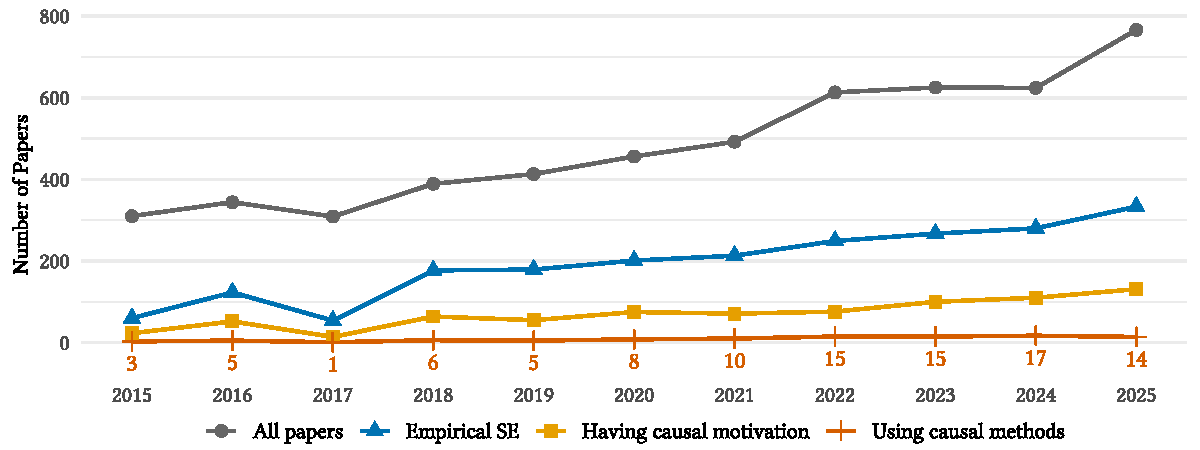
\includegraphics[width=\columnwidth]{figs-tutorial/causal_trends.pdf}
\caption{Publication trends at ICSE, FSE, and ASE (2015--2025).
The top two lines show total publications and empirical SE papers; the bottom two show papers having a causal motivation versus papers employing causal inference methods.
The persistent gap between RQs and methods quantifies the disconnect between causal ambition and methodological practice.}
\label{fig:causal-trends}
\end{figure}

\paragraph{Which Causal Methods Are Used?}
Among the papers with causal methods, the distribution is highly concentrated (Table~\ref{tab:taxonomy}).
Randomized controlled experiments dominate (37 papers), reflecting the SE community's established tradition of controlled developer studies~\cite{DBLP:books/sp/WohlinRHORW24}.
Causal fault localization---applying causal testing, causal contribution scores, or causal debugging to identify root causes of failures---accounts for 13 papers, representing a research thread that applies causal reasoning to software analysis rather than to empirical research methodology.
Regression-based causal inference (14 papers) includes studies that use regression or observational analysis with explicit causal intent, such as controlling for confounders or using causal-adjacent language, but without formal identification strategies.

\begin{table}[t]
\centering
\caption{Taxonomy of causal methods in 99 SE papers (ICSE + FSE + ASE, 2015--2025) classified as employing a causal inference method.
Each paper is assigned a primary category; multi-label assignments are stored separately in the replication package (Section~\ref{sec:tutorial-data-availability}).}
\label{tab:taxonomy}
\footnotesize
\begin{tabularx}{\linewidth}{@{} l r X @{}}
\toprule
\textbf{Category} & \textbf{$n$} & \textbf{Description} \\
\midrule
\multicolumn{3}{l}{\emph{Experimental}} \\
Randomized Controlled Experiment  & 37 & Random assignment to treatment/control groups \\
\addlinespace
\multicolumn{3}{l}{\emph{Observational --- Design-Based}} \\
Quasi-/Natural Experiment         &  6 & Exploits naturally occurring variation (e.g., case-control, before-after, panel data) \\
Propensity Score Methods          &  1 & Matching or weighting on observed covariates to reduce selection bias \\
\addlinespace
\multicolumn{3}{l}{\emph{Observational --- Graphical / Structural}} \\
Causal Graph / DAG                &  7 & Explicitly constructs a directed acyclic graph of assumed causal relationships \\
Causal Discovery                  &  3 & Algorithmically learns causal structure from data \\
Interventional / do-Calculus      &  4 & Estimates effects via Pearl's do-operator or explicit interventions \\
Structural Equation Modeling      &  2 & System of equations with observed/latent variables for direct and indirect effects \\
\addlinespace
\multicolumn{3}{l}{\emph{Observational --- Other}} \\
Counterfactual Analysis           &  7 & Reasons about outcomes under hypothetical alternative conditions \\
Granger Causality                 &  2 & Tests whether past values of one time series predict another \\
Causal Impact Analysis            &  1 & Bayesian structural time-series model for event effects \\
Survival / Hazard Modeling        &  2 & Time-to-event models with causal interpretation \\
Regression-based Causal Inference & 14 & Regression with explicit causal intent but no formal identification strategy \\
\addlinespace
\multicolumn{3}{l}{\emph{Software Analysis (not Empirical Methodology)}} \\
Causal Fault Localization         & 13 & Causal testing, contribution scores, or causal debugging for root-cause analysis \\
\bottomrule
\end{tabularx}
\end{table}

The methods central to the credibility revolution in economics and political science are nearly absent.
Only 6 papers employ quasi-experimental or natural experiment designs; propensity score methods and difference-in-differences are used at most a few times; and no paper in our corpus uses instrumental variables or regression discontinuity as a primary identification strategy.\footnote{A small number of SE studies label their design as ``regression discontinuity'', including the authors' own prior work---e.g., \citet{DBLP:conf/wcre/CasseeVS20} on CI adoption and code reviews, \citet{DBLP:journals/tse/HeHZZ23} on Dependabot adoption---but these use \emph{time} as the running variable, with all units experiencing the treatment simultaneously at a calendar cutoff.
As \citet{hausman2018regression} discuss, such temporal designs are more accurately characterized as \emph{interrupted time series} (ITS) analyses: True regression discontinuity exploits quasi-random variation near a threshold of a continuous assignment variable, whereas ITS designs face confounding from concurrent events and lack the cross-sectional variation that gives RDD its identification power.}
The graphical causal model tradition is better represented (7 papers using causal DAGs, 3 using causal discovery algorithms, 4 using interventional or do-calculus reasoning), consistent with \citeauthor{DBLP:journals/infsof/Siebert23}'s~\cite{DBLP:journals/infsof/Siebert23} observation that Pearl's framework has gained some traction in SE\@.
Structural equation modeling (2 papers), Granger causality (2 papers), and causal impact analysis (1 paper) round out the remaining categories.

\paragraph{Implications.}
This analysis reveals that when SE researchers employ causal methods, they overwhelmingly use randomized controlled experiments, regression-based causal inference, or causal fault localization, with the remaining realms of causal inference (e.g., design-based identification, causal DAGs, structural equation modeling) largely unexplored.
Notably, there are ample opportunities to explore design-based methods that powered the credibility revolution (e.g., difference-in-differences, instrumental variables, regression discontinuity, and panel fixed effects), given the field's abundance of panel data (repositories with temporal structure, developers contributing across projects, tools adopted in staggered fashion) that is well suited to these methods.
Most importantly, we observe a gap between causal ambition and causal methods in empirical SE, and the room for improvement is huge.
This tutorial aims to bridge this gap.

\section{A Primer on Causal Inference for Software Engineering Researchers}
\label{sec:primer}

Our review in Section~\ref{sec:background} shows that, while the causal inference toolkit has matured over a century of cross-disciplinary development into a set of principled methods for answering intervention-outcome questions, fewer than 2\% of SE papers employ any recognized causal inference method despite 29\% carrying an ambition to investigate intervention-outcome questions.
In this section, we will introduce the reader to the conceptual and technical foundations that we believe should be useful to close that gap.
We cover the three pillars most relevant to empirical SE research---counterfactual reasoning and potential outcomes, graphical causal models, and design-based identification---and argue for a pragmatic synthesis suited to the field's observational data.
Due to space constraints, we do not cover advanced topics and recent emerging research directions, such as causal discovery algorithms~\cite{journals/ese/HulseEM25}, machine-learning-based heterogeneous treatment effect estimation~\cite{chernozhukov2018double, athey2016recursive}, and formal verification of causal claims~\cite{halpern2016actual}; readers interested in these topics should consult the references cited and the textbooks listed in Section~\ref{sec:bg-causal-history}.

Throughout this section, we use a few causal inference terms with technical precision.
The \emph{estimand} is the population quantity a study aims to learn; the \emph{estimator} is the procedure (e.g., a regression coefficient, a matched-pair difference) that maps data to a number; and the \emph{estimate} is the specific number that procedure produces on a particular sample.
\emph{Identification} is the bridge between them---the conditions under which the estimator's expected output equals the estimand---and these conditions are made concrete through a set of \emph{identifying assumptions} (random assignment, conditional ignorability, parallel trends, etc.) that the researcher argues for using domain knowledge and features of the research design.
When the identifying assumptions fail, the resulting systematic gap between the estimator's expected output and the estimand is called \emph{bias}, and no amount of data corrects for it.
Table~\ref{tab:glossary} compiles these and other recurring terms into a compact reference for the rest of this section.

\begin{table}[t]
\centering
\caption{Compact glossary of recurring causal inference terms used in this chapter.
The ``See'' column points to the section that introduces each term in detail.}
\label{tab:glossary}
\footnotesize
\begin{tabularx}{\linewidth}{@{} p{3.0cm} X p{1.5cm} @{}}
\toprule
\textbf{Term} & \textbf{Plain-English Description} & \textbf{See} \\
\midrule
Estimand & The population quantity a study aims to learn (the target). & \S\ref{sec:primer} \\
Estimator & A procedure that maps a dataset to a number (the recipe). & \S\ref{sec:primer} \\
Estimate & The specific number produced by running an estimator on a sample. & \S\ref{sec:primer} \\
Identification & The conditions under which the estimator's expected output equals the estimand. & \S\ref{sec:primer} \\
Identifying assumption & A specific, study-level claim that secures identification (e.g., random assignment, parallel trends). & \S\ref{sec:primer} \\
Bias & The systematic gap between an estimator's expected output and the estimand when identifying assumptions fail. & \S\ref{sec:primer} \\
\addlinespace
Potential outcome & The would-have-been outcome of a unit under a given treatment status ($Y(1)$, $Y(0)$). & \S\ref{sec:primer-po} \\
ATE & Average treatment effect across the entire population. & \S\ref{sec:primer-po} \\
ATT & Average treatment effect among units that actually received treatment. & \S\ref{sec:primer-po} \\
\addlinespace
Confounder & A common cause of treatment and outcome that creates spurious association. & \S\ref{sec:primer-dags} \\
Mediator & A variable on the causal pathway from treatment to outcome. & \S\ref{sec:primer-dags} \\
Collider & A common effect of two variables; conditioning on it opens a spurious path. & \S\ref{sec:primer-dags} \\
DAG & Directed acyclic graph encoding the assumed causal structure among variables. & \S\ref{sec:primer-dags} \\
\addlinespace
Conditional ignorability & Identifying assumption for regression, matching, and IPW: treatment is independent of potential outcomes given the observed covariates. & \S\ref{sec:primer-po} \\
Parallel trends & Identifying assumption for difference-in-differences: absent treatment, treated and control groups would have followed the same outcome trajectory. & \S\ref{sec:primer-design} \\
SUTVA & Stable Unit Treatment Value Assumption: no interference between units and a well-defined treatment. & \S\ref{sec:primer-po} \\
Target trial & The hypothetical randomized experiment that an observational study attempts to emulate. & \S\ref{sec:guide-question} \\
\bottomrule
\end{tabularx}
\end{table}

\subsection{What Does It Mean Exactly for X to Cause Y?}
\label{sec:primer-causality}

Consider a question that is highly relevant to SE research: Does adopting AI coding tools increase a project's development velocity?
At its core, this is a question about a contrast between two worlds---one in which a project adopts AI coding tools and one in which it does not---and whether development velocity differs between them.
This deceptively simple framing conceals a deep conceptual question: What does it \emph{mean} for one thing to cause another?
Two perspectives---one abstract, one operational---provide the conceptual foundation for the toolkit introduced in this section.\footnote{The most intuitive philosophical account, dating to \citet{hume1748enquiry}, holds that $X$ causes $Y$ if $X$ is regularly followed by $Y$---but regular association cannot distinguish genuine causal effects from systematic differences between compared groups (Section~\ref{sec:primer-naive} makes this failure concrete), motivating the more rigorous perspectives below.
A complementary \emph{interventionist} account, developed by \citet{woodward2003making} and formalized through \citeauthor{pearl2009causality}'s~\cite{pearl2009causality} do-calculus, underpins the graphical causal model framework and is introduced alongside DAGs in Section~\ref{sec:primer-dags}.}

\paragraph{Causation as Counterfactual Dependence.}
The formal foundation of modern causal inference, developed by \citet{rubin1974estimating} building on philosophical work by \citet{lewis1973causation}, defines causation through \emph{counterfactuals}: $X$ causes $Y$ if $Y$ would not have occurred (or would have differed) had $X$ not occurred.
Applied to our example: AI tools \emph{caused} the velocity increase for a given project if that project \emph{would have had lower development velocity} had it not adopted AI tools, all else being equal.
This definition is precise but introduces what \citet{holland1986statistics} called the \emph{fundamental problem of causal inference}: We can never observe both worlds for the same unit.
We observe the project's development velocity after adopting AI tools, or its velocity without AI tools, but never both.
The entire apparatus of causal inference---from randomized experiments to quasi-experimental designs---exists to overcome this fundamental observational limitation.
Still, the counterfactual view is useful in that it helps the researcher derive \emph{estimands}---precise definitions of the causal quantities we seek to estimate---and is formalized through the potential outcomes framework (Section~\ref{sec:primer-po}).

\paragraph{Causation as Three Necessary Conditions.}
A classical perspective on causation, with origins in \citet{hill1965environment} and formalized for modern observational studies by \citet{rosenbaum2002observational} and \citet{shadish2002experimental}, requires three conditions for a causal relationship to hold: \emph{temporal precedence} (the cause must precede the effect), \emph{empirical association} (a statistical relationship between cause and effect must be observable), and \emph{non-spuriousness} (the relationship must not be explained by confounding variables).
This framing is the operational definition taught in graduate empirical SE methodology courses~\cite{vasilescu17803} and underpins a growing line of cohort-style observational studies in SE~\cite{DBLP:conf/esem/SaarimakiLVJ020}.
Each condition maps to a distinct concern that the causal inference toolkit addresses: Temporal precedence motivates longitudinal and panel designs (Sections~\ref{sec:primer-design} and~\ref{sec:longitudinal}); empirical association is what statistical estimators recover under correct specification; and non-spuriousness is the target of both covariate adjustment justified by graphical causal models (Section~\ref{sec:primer-dags}) and design-based identification strategies (Section~\ref{sec:primer-design}).
The three conditions are necessary but not sufficient---they can be derived as consequences of the counterfactual framework---and serve as a practical checklist for the empirical researcher to evaluate whether their observational design has a chance of supporting a causal claim.

Together, these two perspectives motivate the three technical pillars of modern causal inference introduced in Section~\ref{sec:primer-toolkit}: potential outcomes formalize the counterfactual view (Section~\ref{sec:primer-po}), graphical causal models encode the structural assumptions that determine when the three conditions can be jointly satisfied (Section~\ref{sec:primer-dags}), and design-based identification exploits quasi-random variation in the observational setting to approximate the temporal precedence and non-spuriousness conditions that pure covariate adjustment often cannot deliver (Section~\ref{sec:primer-design}).

\subsection{Why Cannot We Use Descriptive and Correlational Evidence?}
\label{sec:primer-naive}

Before introducing the toolkit, we must understand why the approaches dominant in SE research fail to convincingly establish causation.
Two common strategies---comparing outcomes across groups and adding regression controls---each fall short in ways that motivate the formal machinery in Sections~\ref{sec:primer-toolkit}.

Consider the AI tools question again: Suppose a researcher compares monthly commits in a group of projects that adopted AI coding tools against a group of projects that did not and finds that AI-adopting projects have more commits.
Can this comparison support the claim that AI tools \emph{cause} higher development velocity?
It is highly questionable, because the two groups were never comparable to begin with.
It is very likely that projects that adopt AI coding tools differ systematically from those that do not---they may be using more AI-friendly programming languages (e.g., TypeScript and Python), have more active maintainers, more community attention, more disciplined development practices, and may belong to organizations that invest more in developer productivity.
These characteristics are \emph{confounders}: They influence both the decision to adopt AI tools (the treatment) and development velocity (the outcome), creating an association between AI tools and higher velocity even if the tools themselves have zero causal effect.
The observed difference in commit rates is a mixture of any genuine AI tool effect and the \emph{selection bias} arising from systematic differences between the compared groups---and a simple group comparison cannot disentangle the two.

The natural response is to control for these confounders using multivariate regression---e.g., one with project age, project size, number of contributors, and other covariates---and interpret the remaining coefficient on AI tool adoption as the causal effect.
This strategy is by far the most common approach to causal questions in empirical SE research, yet it suffers from at least four distinct problems plaguing many observational studies:
\begin{itemize}[leftmargin=15pt]
    \item \emph{Unobserved Confounders.}
    Regression can only adjust for measured variables, yet many confounders that plausibly affect both AI tool adoption and development velocity---e.g., developer expertise, team culture, organizational practices, project management quality---are largely unmeasurable from repository data.
    No amount of observed controls can compensate for these missing variables, and the resulting bias can be large in either direction.\footnote{Formally, if the true causal model includes an unobserved confounder $U$, the regression coefficient on the treatment converges to $\hat{\tau} \xrightarrow{p} \tau + \gamma \cdot \text{Cov}(D, U|X) / \text{Var}(D|X)$, where $\gamma$ is the effect of $U$ on the outcome and $\text{Cov}(D, U|X)/\text{Var}(D|X)$ captures the residual association between treatment and the omitted variable after partialling out the included controls (see~\citet[Ch.~3, \S3.2.2]{angrist2009mostly} for a formal derivation and \citet{cinelli2020making} for a modern sensitivity-analysis extension).
    The bias is large whenever $U$ strongly predicts both treatment $D$ and outcome $Y$.}
    \item \emph{Collider Bias.}
    When a variable is a common \emph{effect} of both treatment and outcome, conditioning on it in a regression creates spurious associations.
    For example, if GitHub popularity (e.g., star count) is influenced by both AI tool adoption (early adopters attract attention) and development velocity (active projects gain visibility), a regression with popularity as a control can manufacture an apparent relationship between AI tools and development velocity even where none exists in the full population.\footnote{In a causal directed acyclic graph (DAG), a \emph{collider} is a variable with two or more incoming arrows (e.g., $X \to C \leftarrow Y$).
    Marginally, $X$ and $Y$ may be independent, but conditioning on $C$ ``opens'' the path between them, inducing a spurious association---an effect sometimes called Berkson's paradox~\cite{berkson1946limitations}.
    Intuitively, once we know the value of a common effect, learning about one cause provides information about the other: Among popular projects, if a project did \emph{not} benefit from AI tool adoption (and its associated visibility), it likely achieved popularity through high development velocity, creating a negative association between AI adoption and development velocity that is purely an artifact of the conditioning.
    See Section~\ref{sec:primer-dags} for more details on DAGs, \citet[Ch.~1, \S1.2.3]{pearl2009causality} for the formal $d$-separation proof, and \citet{elwert2014endogenous} for an accessible treatment with social-science examples.}
    \item \emph{Mediator Bias.}
    When a variable lies \emph{on the causal pathway} from treatment to outcome, conditioning on it in a regression blocks part of the genuine effect.
    For example, if AI coding tools increase development velocity partly by automating code review and accelerating pull request throughput, then controlling for PR throughput attenuates or eliminates the very signal the researcher seeks to detect.\footnote{Formally, if the causal structure is $X \to M \to Y$ (treatment affects outcome through mediator $M$), conditioning on $M$ removes the indirect effect and leaves only the direct effect $X \to Y$.
    When the entire effect operates through the mediator---as may be the case if AI tools' velocity benefit operates entirely through faster code generation---conditioning on $M$ makes the effect vanish entirely, even though the treatment genuinely causes the outcome.
    The researcher who targets the \emph{total} effect of $X$ on $Y$ should therefore not condition on any variable on the causal pathway.
    Similarly, see \citet[Ch.~3, \S3.3.1]{pearl2009causality} for the formal derivation via the back-door criterion and \citet{wysocki2022statistical} for a demonstration of this error in applied research.}
    \item \emph{Reverse Causality.}
    Finally, regression on cross-sectional data (i.e., data collected at a single point in time) cannot determine whether AI tools increase development velocity or whether already-high-velocity teams are the ones that adopt AI tools; no set of cross-sectional controls can distinguish these two causal directions.
    Section~\ref{sec:temporal-collapse} formalizes this problem as \emph{temporal collapse}: When a cross-sectional snapshot collapses time-indexed variables into atemporal summaries, the resulting graph is cyclic and no valid adjustment set exists.
\end{itemize}
Despite these concerns, multivariate regression is not inherently incapable of supporting causal claims---under specific conditions, it can be a valid identification strategy~\cite{angrist2009mostly, cunningham2021causal}.
However, determining whether those conditions hold requires the formal frameworks introduced in Section~\ref{sec:primer-toolkit}: The \emph{potential outcomes framework} (Section~\ref{sec:primer-po}) defines precisely what causal quantity the researcher seeks to estimate, and the \emph{graphical causal model} framework (Section~\ref{sec:primer-dags}) provides a principled basis---through the \emph{back-door criterion}---for determining which covariates must be included, which must be excluded, and whether the remaining assumptions are plausible.
We defer the technical details to those sections, where the formalisms make the conditions precise and where design-based alternatives (Section~\ref{sec:primer-design}) offer a path forward for the many SE settings in which the regression requirements cannot be plausibly met.

\subsection{The Causal Inference Toolkit}
\label{sec:primer-toolkit}

Applied causal inference rests on three complementary pillars, each addressing a distinct question.
\emph{Potential outcomes} answer: What do we want to estimate?
They provide a formal language for defining causal estimands---the ATE, ATT, LATE---independently of any statistical model.
\emph{Graphical causal models} answer: What must we assume about the world for our estimate to be valid?
They encode causal assumptions as directed acyclic graphs (DAGs), making every assumption visible and debatable.
\emph{Design-based identification} answers: How can we exploit features of the research setting to make those assumptions credible?
Methods such as difference-in-differences, instrumental variables, and regression discontinuity derive identification from quasi-random variation rather than from the hope that all confounders have been measured.
Modern applied researchers use all three together: Potential outcomes define the target, DAGs encode the assumed causal structure, and design-based methods provide the identification strategy.

\subsubsection{The Potential Outcomes Framework}
\label{sec:primer-po}

The potential outcomes framework~\cite{neyman1923application, rubin1974estimating} formalizes the counterfactual view of causation introduced in Section~\ref{sec:primer-causality} and operationalizes the \emph{estimand-first} principle~\cite{lundberg2021estimand}: Before choosing a statistical method, the researcher must first define the causal quantity of interest.
In this section, we formally introduce this framework in the simplest binary treatment case and highlight its mathematical power in transparently articulating the \emph{identifying assumptions} needed for the estimates to carry a causal interpretation.

\paragraph{Notation and Setup.}
In the binary treatment case, each study unit $i$ has two \emph{potential outcomes}: $Y_i(1)$ under treatment and $Y_i(0)$ without treatment.
The individual causal effect $\tau_i = Y_i(1) - Y_i(0)$ is unobservable because only one potential outcome is realized---the fundamental problem of causal inference discussed in Section~\ref{sec:primer-causality}.

\paragraph{Causal Estimands.}
To get over this problem, researchers seek to estimate \emph{population-level summaries}.
One option is the \emph{Average Treatment Effect} (ATE), $\text{ATE} = E[Y(1)] - E[Y(0)]$, which answers questions like: On average across \emph{all} projects, how much does adopting AI coding tools change development velocity?
Another option is the \emph{Average Treatment Effect on the Treated} (ATT), $\text{ATT} = E[Y(1) - Y(0) \mid D = 1]$, which answers questions like: Among projects that \emph{actually adopted} AI coding tools, how much did adoption change their development velocity?
ATE and ATT coincide only under homogeneous effects or independence of treatment assignment.
Other estimands include the \emph{Local Average Treatment Effect} (LATE) for the subpopulation affected by an instrument, and \emph{conditional average treatment effects} (CATEs), $\tau(x) = E[Y(1) - Y(0) \mid X = x]$, for subgroups defined by covariates~$X$.\footnote{The LATE theorem, which shows that instrumental variables identify the causal effect for the subpopulation of \emph{compliers}, was introduced by \citet{angrist1996identification}; see \citet[Ch.~4, \S4.4--4.5]{angrist2009mostly} for a textbook treatment.
For CATEs and effect heterogeneity more broadly, a growing literature develops machine-learning estimators: \emph{Causal forests}~\cite{athey2016recursive, wager2018estimation} adapt random forests to estimate $\tau(x)$ under conditional ignorability, and \emph{double/debiased machine learning}~\cite{chernozhukov2018double} enables flexible nuisance-function estimation while preserving valid statistical inference.
These methods extend rather than replace the identification frameworks discussed in this section: A causal forest trained on data with unmeasured confounders produces biased CATE estimates, not unbiased ones.
We therefore treat effect heterogeneity as a secondary concern downstream of identification; see \citet[Ch.~10]{huntingtonklein2021effect} for an accessible introduction and Appendix~\ref{sec:appendix-faq} for further discussion.}
Which estimand to target is a substantive decision, not a statistical one: The researcher must decide whether the question concerns the average effect across all projects (ATE), the effect on adopters (ATT), the effect on the subpopulation induced to adopt by a specific mechanism (LATE), or the heterogeneity of effects across different subgroups (CATEs).

One particular power of the potential outcomes formalism is that it allows researchers to derive the \emph{identifying assumptions} required for the study's results to have a causal interpretation.
For example, in a \emph{randomized controlled trial} (RCT), the formal identifying assumption is that treatment is statistically independent of the potential outcomes (i.e., treatment is as-if randomly assigned, written $(Y(1), Y(0)) \perp D$), so selection bias vanishes and the naive comparison identifies the ATE\@.
A valid RCT additionally requires the \emph{Stable Unit Treatment Value Assumption} (SUTVA), i.e., no interference between units and a well-defined treatment, and \emph{full compliance}, i.e., the research units are truly following their assigned treatment status.
For the family of regression, matching, and inverse probability weighting methods (for which we jointly refer to as the \emph{selection-on-observables} family), the formal identifying assumption is \emph{conditional ignorability}---the assumption that, conditional on observed covariates $X$, treatment assignment is independent of potential outcomes: $(Y(1), Y(0)) \perp D \mid X$.
Under this assumption, plus overlap ($0 < P(D\!=\!1 \mid X\!=\!x) < 1$ for all $x$ in the support of $X$), the ATE is identified through differencing the predicted outcome based on $X$:
In practice, this assumption means that all confounders must be captured in $X$ for the regression to produce a credible causal estimate, whose plausibility can be assessed through the graphical causal framework (Section~\ref{sec:primer-dags}) and complementary sensitivity analysis.\footnote{For textbook proofs that randomization identifies the ATE and that conditional ignorability identifies the ATE via regression, see \citet[Ch.~2]{angrist2009mostly} and \citet[Chs.~2--3]{hernan2020causal}.
Several methods exist to probe whether the conditional ignorability assumption is plausible:
\emph{Rosenbaum bounds}~\cite{rosenbaum2002observational} quantify how strong an unmeasured confounder would have to be to alter the study's conclusions;
\emph{coefficient stability}~\cite{oster2019unobservable} assesses whether point estimates shift substantially as controls are added, with large shifts suggesting important omitted variables;
the \emph{E-value}~\cite{vanderweele2017sensitivity} reports the minimum strength of association an unmeasured confounder would need with both treatment and outcome to explain away an observed effect;
and the \emph{robustness value}~\cite{cinelli2020making} generalizes this logic to partial $R^2$ measures, indicating how much residual variation a confounder must explain to nullify the result.
None of these methods can \emph{prove} that all confounders are measured, but they transform the unverifiable assumption into a quantitative question---\emph{how much} confounding would be required---that reviewers and readers can evaluate against in a specific setting using their domain knowledge.}

\subsubsection{Graphical Causal Models and DAGs}
\label{sec:primer-dags}

For the selection-on-observables family of methods---regression, matching, inverse probability weighting---the potential outcomes framework defines the estimand but offers limited guidance on \emph{which} variables to condition on.
As Section~\ref{sec:primer-naive} illustrated, conditioning on the wrong variables can introduce bias rather than remove it.
\citeauthor{pearl2009causality}'s~\cite{pearl2009causality} graphical framework addresses this gap through an \emph{interventionist} view of causation~\cite{woodward2003making}: $X$ causes $Y$ if intervening on $X$---holding everything else fixed---changes $Y$.
Pearl formalizes this through the \emph{do-operator}, contrasting $P(Y \mid X\!=\!1)$---the conditional probability of $Y$ among units where $X$ happens to equal 1---with $P(Y \mid do(X\!=\!1))$---the probability of $Y$ when the researcher intervenes to set $X$ equal to 1.
The two quantities differ whenever the association between $X$ and $Y$ is partially driven by common causes rather than by $X$ itself, and the central question of causal inference is precisely when observational data alone suffices to identify the interventional quantity.
\emph{Directed acyclic graphs} (DAGs) encode the qualitative causal structure that determines when this identification is possible, providing the bridge between the data we observe and the interventions we wish to reason about.

\paragraph{Directed Acyclic Graphs.}
A DAG encodes \emph{the researcher's beliefs about the true data-generating process} and it consists of nodes (variables) and directed edges ($\to$) representing direct causal effects.
Every arrow is a substantive claim; every absent arrow asserts no direct effect.
This transparency is the central value of DAGs for applied research: Rather than debating vaguely about ``omitted variables'' or ``lurking confounders,'' researchers can argue about specific edges.

\paragraph{Constructing a DAG from Prior Theory.}
To make the discipline of theory-driven DAG construction concrete, we anchor each node in Figure~\ref{fig:ai-dag} in the relevant prior literature, keeping the figure deliberately small (one mediator, one collider) so that every claim is traceable.
\emph{Code Generation} is the mediator because randomized experiments document that AI tools accelerate per-task code production~\cite{cui2025effects, DBLP:journals/corr/abs-2302-06590, DBLP:conf/icse-seip/ParadisGMNMMZFC25}.
\emph{Popularity} is the collider because visibility on GitHub responds causally to external shocks~\cite{DBLP:conf/icse/FangLHV22}, and the same symmetry applies to AI adoption and to high development velocity, so both feed into the same node.
\emph{Project Maturity} and \emph{Domain} (primary programming language) are observable pre-treatment confounders, consistent with the practitioner observation that AI tools work unevenly across language ecosystems and that younger projects are typical early adopters; their imbalance across treated and control groups is documented descriptively in Section~\ref{sec:naive-comparison}.
\emph{Team Skill}---encompassing developer expertise, team culture, and organizational practice---is the canonical unobserved confounder, since GitHub repository data captures no proxy for it; Figure~\ref{fig:ai-dag} marks it with a dashed border, and Section~\ref{sec:cross-sectional-sensitivity} shows that the cross-sectional estimate is highly sensitive to its plausible magnitude.
Other mediators (e.g., workflow automation, code review acceleration) and confounders (e.g., team size, organization ownership) are plausible but omitted from the pedagogical figure; the temporal DAG in Section~\ref{sec:temporal-dag} reintroduces the time-varying ones in their proper temporal incarnations.\footnote{The sharp reader may have already noticed the fact that the DAG presented in Figure~\ref{fig:ai-dag} is ambiguous without considering the temporal nature of software engineering data: For example, the number of stars received can be a confounder \emph{before} AI tools adoption (more popular projects both exhibit higher velocity and are more likely to adopt AI tools) and a collider \emph{after} AI tools adoption (higher-velocity and AI-enabled projects are more likely to receive more stars).
We construct the proper temporal DAG and diagnose this problem formally in Section~\ref{sec:temporal-dag}.}

\begin{figure}[t]
\centering
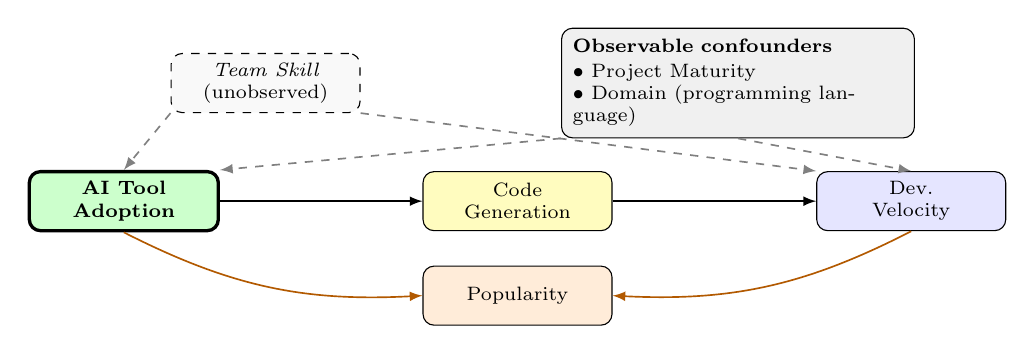
\begin{tikzpicture}[
    >=latex, font=\scriptsize,
    confbox/.style={draw, rounded corners, fill=gray!12, align=left,
                    text width=4.2cm, inner sep=4pt},
    tnode/.style={draw, rounded corners, fill=green!20, very thick,
                  minimum height=0.75cm, minimum width=2.4cm,
                  align=center, font=\bfseries\scriptsize},
    mnode/.style={draw, rounded corners, fill=yellow!25,
                  minimum height=0.75cm, minimum width=2.4cm, align=center},
    ynode/.style={draw, rounded corners, fill=blue!10,
                  minimum height=0.75cm, minimum width=2.4cm, align=center},
    cnode/.style={draw, rounded corners, fill=orange!15,
                  minimum height=0.75cm, minimum width=2.4cm, align=center},
    unobs/.style={draw, rounded corners, dashed, fill=gray!5,
                  minimum height=0.75cm, minimum width=2.4cm, align=center,
                  font=\itshape\scriptsize},
    cedge/.style={->, gray, dashed, semithick},
    medge/.style={->, black, semithick},
    coledge/.style={->, orange!70!black, semithick},
]
% Top row: unobserved + observable confounders
\node[unobs] (skill) at (1.8, 1.5) {Team Skill\\\emph{(unobserved)}};
\node[confbox] (Conf) at (7.8, 1.5) {%
    \textbf{Observable confounders}\\[1pt]
    $\bullet$ Project Maturity\\
    $\bullet$ Domain (programming language)
};

% Middle row: causal chain
\node[tnode] (D) at (0, 0) {AI Tool\\Adoption};
\node[mnode] (M) at (5, 0) {Code\\Generation};
\node[ynode] (Y) at (10, 0) {Dev.\\Velocity};

% Bottom row: collider
\node[cnode] (C) at (5, -1.2) {Popularity};

% Back-door edges (dashed gray)
\draw[cedge] (skill.south west) -- (D.north);
\draw[cedge] (skill.south east) to (Y.north west);
\draw[cedge] (Conf.south west) to (D.north east);
\draw[cedge] (Conf.south) -- (Y.north);

% Causal mechanism (solid black)
\draw[medge] (D) -- (M);
\draw[medge] (M) -- (Y);

% Collider edges (solid orange)
\draw[coledge] (D.south) to[bend right=15] (C.west);
\draw[coledge] (Y.south) to[bend left=15] (C.east);
\end{tikzpicture}
\caption{An example DAG for the AI coding tools and development velocity question, with each node anchored in the literature cited in the text.
Solid black arrows trace the identified causal path: AI Tool Adoption $\to$ Code Generation $\to$ Dev.\ Velocity.
Dashed gray arrows mark back-door paths through the three confounders---two observable (Project Maturity, Domain) and one unobserved (Team Skill, dashed border)---each of which a valid selection-on-observables analysis must block by conditioning on the observable ones and sensitivity-analyzing the unobservable one.
Solid orange arrows mark the collider relationship around Popularity (AI Tool Adoption $\to$ Popularity $\leftarrow$ Dev.\ Velocity); conditioning on Popularity \emph{opens} this back-door path rather than closing it.}
\label{fig:ai-dag}
\end{figure}

\paragraph{Back-Door Paths and the Back-Door Criterion.}
In a DAG, \emph{causal paths} follow arrows from treatment to outcome; in Figure~\ref{fig:ai-dag}, the causal path runs AI Tool Adoption $\to$ Code Generation $\to$ Dev.\ Velocity.
This path transmits the genuine causal effect.
A \emph{back-door path}, by contrast, connects treatment to outcome through a common cause without following the direction of the arrows---for example, AI Tool Adoption $\leftarrow$ Team Skill $\rightarrow$ Dev.\ Velocity.
These back-door paths transmit spurious associations: Even if AI tools had zero effect on Dev.\ Velocity, the fact that skilled teams both adopt AI tools earlier and inherently exhibit higher velocity creates an observed correlation between AI adoption and development velocity.
A naive comparison conflates the genuine causal effect that flows through the causal paths with the spurious associations that flow through the back-door paths.

The \emph{back-door criterion}~\cite{pearl2009causality} provides a principled rule for which variables to condition on in order to block all back-door paths without inadvertently blocking the causal paths.
A set $Z$ satisfies the criterion if (1)~no variable in $Z$ is a descendant of the treatment, and (2)~conditioning on $Z$ blocks every back-door path.
In Figure~\ref{fig:ai-dag}, $Z = \{\text{Team Skill},\, \text{Project Maturity},\, \text{Domain}\}$ satisfies this criterion: Each is a common cause of AI Tool Adoption and Dev.\ Velocity, and conditioning on all three blocks every back-door path; however, Team Skill is unobserved, so the feasible adjustment set is $Z_{\text{obs}} = \{\text{Project Maturity},\, \text{Domain}\}$, and the residual confounding from the unblocked Team Skill back-door must be addressed through sensitivity analysis (Section~\ref{sec:cross-sectional-sensitivity}) rather than conditioning.
Two types of variables must \emph{not} be included in $Z$.
Code Generation is a \emph{mediator} on the causal path: Conditioning on it blocks the very effect the researcher seeks to estimate.
Popularity is a \emph{collider}: Conditioning on it \emph{opens} a spurious path rather than closing one.
When $Z$ satisfies the back-door criterion, it provides a justifiable basis that a selection-on-observables method satisfies the conditional ignorability assumption derived from the potential outcomes framework (Section~\ref{sec:primer-po}).

\paragraph{Limitations of DAGs.}
DAGs require \emph{domain knowledge} to construct---they encode the researcher's assumptions about the data-generating process, not knowledge derived from the data itself.\footnote{Causal discovery algorithms~\cite{spirtes2001causation} attempt to learn DAG structure directly from data, but they require their own strong assumptions (faithfulness, causal sufficiency) and remain fragile in practice.
In SE specifically, \citet{journals/ese/HulseEM25} showed that causal graph generators are unstable, with over half the discovered edges changing across minor data perturbations.
We take the stance that domain knowledge remains essential for constructing credible DAGs, though data-driven methods are an important research frontier that can complement expert judgment by suggesting edges to investigate.}
Further, a DAG's validity depends on the completeness of the variables included; omitting an important confounder renders the back-door criterion unreliable.\footnote{Sensitivity analysis tools partially address this limitation by quantifying how strong an unmeasured confounder would need to be to alter a study's conclusions---see Rosenbaum bounds~\cite{rosenbaum2002observational}, coefficient stability~\cite{oster2019unobservable}, and the robustness value~\cite{cinelli2020making}, discussed in detail in Section~\ref{sec:primer-po}.}
Finally, DAGs encode qualitative causal structure (which variables affect which) but say nothing about the \emph{magnitude} or functional form of effects.\footnote{Pearl's broader structural causal model framework~\cite{pearl2009causality} augments the qualitative DAG with functional equations and derives nonparametric identification formulas, and semiparametric estimators such as double/debiased machine learning~\cite{chernozhukov2018double} can then estimate these quantities without imposing strong functional form assumptions, bridging the gap between qualitative causal structure and quantitative effect estimation.}
Despite these limitations, DAGs remain the most practical tool for making causal assumptions transparent and debatable~\cite{rohrer2018thinking, tennant2021dags}.
For selection-on-observables methods, DAGs are indispensable: The back-door criterion provides the only principled basis for deciding which covariates to include and which to exclude.
When identification instead derives from features of the research design (Section~\ref{sec:primer-design}), DAGs play a supporting but still valuable role---providing a transparent ground for clarifying which confounders the design absorbs and which still remain as potential threats.

\subsubsection{Design-Based Identification}
\label{sec:primer-design}

The preceding section showed how DAGs guide covariate selection for regression and matching---methods that identify causal effects under the assumption that \emph{all} confounders are observed and adjusted for.
In many SE settings, where key confounders such as developer skill, team culture, and organizational practices are largely unmeasurable from repository data, justifying this assumption is challenging.
\emph{Design-based identification} takes a fundamentally different approach: Rather than attempting to measure and adjust for all confounders, it exploits features of the research setting---temporal variation, natural experiments, assignment thresholds---that provide quasi-random variation in treatment assignment.
This essentially creates a \emph{natural experiment} setting that approximates an idealized randomized comparison~\cite{dunning2012natural,hernan2020causal}.
The credibility of these methods derives not from the completeness of the causal theory but from the transparency and partial testability of their design-specific assumptions~\cite{angrist2010credibility}.

\begin{table}[t]
\centering
\caption{Common causal inference methods, their target estimands, and key identification assumptions under the potential outcomes framework.
ATE = Average Treatment Effect; ATT = Average Treatment Effect on the Treated; LATE = Local Average Treatment Effect.
We use precise terminologies in this table; see the references for detailed explanations of these terminologies.}
\label{tab:methods-summary}
\footnotesize
\begin{tabularx}{\linewidth}{@{} p{3.2cm} p{1.6cm} X @{}}
\toprule
\textbf{Method} & \textbf{Estimand} & \textbf{Key Identification Assumptions} \\
\midrule
Randomized Controlled Trial
  & ATE
  & Random assignment: $(Y(1), Y(0)) \perp D$; SUTVA; full compliance \cite[Ch.~4]{cunningham2021causal} \\
\addlinespace
Selection on Observables {\scriptsize (Regression, Matching, IPW)}
  & ATE / ATT
  & Conditional ignorability: $(Y(1), Y(0)) \perp D \mid X$; overlap; correct functional form for parametric estimators \cite[Ch.~3]{angrist2009mostly}, \cite[Ch.~5]{cunningham2021causal} \\
\addlinespace
Difference-in-Differences
  & ATT
  & Parallel trends: absent treatment, treated and control groups would have followed the same trajectory; no anticipation; SUTVA \cite[Ch.~5]{angrist2009mostly}, \cite[Ch.~9]{cunningham2021causal} \\
\addlinespace
Instrumental Variables
  & LATE
  & Relevance: instrument $Z$ affects treatment; exclusion: $Z$ affects outcome only through treatment; independence; monotonicity (no defiers) \cite[Ch.~4]{angrist2009mostly}, \cite[Ch.~7]{cunningham2021causal} \\
\addlinespace
Regression Discontinuity
  & LATE \scriptsize{(at cutoff)}
  & Continuity of potential outcomes at threshold; no precise manipulation of running variable; no compound treatments at cutoff \cite[Ch.~6]{angrist2009mostly}, \cite[Ch.~6]{cunningham2021causal} \\
\addlinespace
Panel Fixed Effects
  & ATE \scriptsize{(within-unit)}
  & Strict exogeneity: conditional on unit FE, treatment is uncorrelated with time-varying unobservables; no time-varying confounders \cite[Ch.~5]{angrist2009mostly}, \cite[Ch.~8]{cunningham2021causal} \\
%\addlinespace
%Synthetic Control
%  & ATT \scriptsize{(treated unit)}
%  & Synthetic control tracks treated unit's counterfactual trajectory; no interference; no anticipation \\
\bottomrule
\end{tabularx}
\end{table}

Table~\ref{tab:methods-summary} summarizes the methods most relevant to SE research, along with their formal estimand and identifying assumptions derived from the potential outcomes framework (see \citet[Chs.~2--6]{angrist2009mostly} and \citet[Chs.~4--9]{cunningham2021causal} for formal proofs and detailed treatments of each method).
In this section, we illustrate the high-level idea of each method with SE examples to build intuition:

\begin{itemize}[leftmargin=15pt]
    \item \emph{Difference-in-Differences (DiD).}
    DiD compares changes in outcomes over time between a treated group and a control group, e.g., comparing development velocity trends before and after AI tool adoption in treatment repositories versus comparable repositories that did not adopt.
    The key assumption---\emph{parallel trends}---requires that, absent the adoption, both groups would have followed the same outcome trajectory.
    This assumption can be partially assessed using pre-treatment trend tests, and modern estimators leverage staggered adoption to construct natural experiments among treated units with different adoption timings~\cite {callaway2021difference, roth2023whats}.
    The DiD methodology has been successfully applied in SE settings to study the impact of social media promotion on open-source project popularity and contributor attraction~\cite{DBLP:conf/icse/FangLHV22}, the impact of core contributor disengagement on open-source project workflows~\cite{DBLP:conf/icse/ChenSSGT26}, and the impact of Cursor adoption on development velocity and code quality~\cite{DBLP:conf/msr/HeMAKV26}.
    As a tutorial example, we will apply staggered DiD to the AI coding tools question in Section~\ref{sec:did}.

    \item \emph{Instrumental Variables (IV).}
    IV uses an \emph{instrument}---a variable that affects the treatment but influences the outcome only through the treatment---to isolate exogenous variation.
    The IV estimand is the LATE---the effect on units whose treatment status was changed by the instrument~\cite{angrist1996identification}.
    \citet{DBLP:journals/tosem/GrafVlachyW24} provide a comprehensive tutorial on applying IV and two-stage estimation in SE research, using the observed correlation between indentation style (tabs vs. spaces) and developer salary---where programming language acts as an omitted confounder---to illustrate how IV can recover consistent causal estimates when conventional regression is biased by endogeneity.

    \item \emph{Regression Discontinuity (RDD).}
    RDD exploits \emph{sharp} thresholds in treatment assignment to create a quasi-experimental contrast in the outcome between units just above and just below the threshold.
    For example, if open-source projects exceeding a certain popularity threshold are eligible for a sponsorship program, comparing projects just above and just below the threshold provides a quasi-experimental contrast in the program's outcomes.
    Identification requires that potential outcomes are continuous at the threshold and that units cannot precisely manipulate their position relative to the cutoff.
    To our knowledge, we are unaware of a successful RDD application in an SE setting (see previous footnote in Section~\ref{sec:bg-adoption} for a discussion of terminology misuses).

    \item \emph{Panel Fixed Effects.}
    Panel fixed effects models compare repeated observations of the same unit over time, absorbing all \emph{time-invariant} characteristics through unit-specific intercepts.
    For example, observing the same repository before and after AI tool adoption removes confounding from all time-invariant repository characteristics---codebase domain, long-term team composition, organizational practices---that cross-sectional comparisons cannot address.
    The identifying assumption is \emph{strict exogeneity}: Conditional on unit fixed effects, the treatment is uncorrelated with time-varying unobservables (i.e., no time-varying confounders that are left unmeasured).\footnote{This assumption differs from the conditional ignorability assumption from selection-on-observables methods: Panel fixed effects automatically absorb all time-invariant confounders without requiring them to be measured, but the researcher must still argue---using domain knowledge or a DAG---that no unmeasured time-varying confounders remain and that past outcomes do not feed back into future treatment assignment.}
    Panel fixed effects models have been applied in SE settings to study the causal impact of code quality on developer productivity at Google~\cite{DBLP:conf/sigsoft/ChengMCJGKZ022}.
    They are also often used as a baseline model for DiD designs (see Section~\ref{sec:did} for an example).
\end{itemize}

\subsection{A Pragmatic Stance for Software Engineering Research}
\label{sec:primer-stance}
\label{sec:guide}

The preceding subsections introduced a rich but potentially daunting toolkit: Potential outcomes define estimands, DAGs encode mechanisms, and design-based methods exploit quasi-random variation.
An SE researcher encountering these ideas for the first time faces an immediate practical question: \emph{How do I actually use this?}
In general, there is no universal recipe for causal inquiries in \emph{any} research setting---causal inference requires both methodological rigor and creative problem-solving, and the ``right'' approach depends on the specific features of the data and setting.
Drawing on the emerging consensus across econometrics~\cite{imbens2020potential, angrist2010credibility}, epidemiology~\cite{hernan2020causal}, and sociology~\cite{lundberg2021estimand}, we recommend a pragmatic synthesis tailored to the realities of empirical SE research as follows.

\paragraph{Build on Prior Research and Practitioner Knowledge.}
\label{sec:stance-prior-research}
Every step of a causal inquiry---framing the question, proposing a DAG, choosing covariates---requires \emph{domain knowledge} that cannot be derived from the data alone.
In SE, this knowledge comes from three sources.
First, prior quantitative studies provide the raw material for proposing causal structures: An observed association between AI tool adoption and development velocity does not itself establish causation, but it motivates a DAG edge that can then be subjected to rigorous identification.
Second, gray literature---blog posts, postmortems, industry reports, conference talks---encodes rich practitioner causal beliefs (``we adopted X so Y improved'') that inform which mechanisms are plausible and which confounders are likely.
Third, qualitative SE research---interviews, case studies, grounded theory---surfaces causal reasoning that developers and teams use in practice, providing mechanistic accounts that purely quantitative data cannot.
These sources collectively generate the theories that causal methods then test, creating a virtuous cycle: Prior work proposes causal structures, rigorous methods evaluate them, and the findings refine theory for the next iteration.

\paragraph{Use Counterfactual Reasoning to Frame Research Designs.}
\label{sec:guide-question}
Before analyzing data, think about the \emph{target trial}~\cite{hernan2020causal}: Every causal question implicitly describes a hypothetical randomized experiment, and naming that concretely is the most effective way to expose what an observational study is actually trying to estimate.
What is the treatment, the population, the outcome, and the timing?
This exercise forces clarity about aspects that SE studies often leave implicit---for example, whether ``AI tool adoption'' refers to code generation, automated review, or the broader workflow changes that accompany the tools.
For the AI coding tools question, the target trial would randomly assign a set of comparable software projects to adopt AI coding tools and compare a chosen velocity outcome after a fixed period.
Articulating this trial immediately reveals threats to validity that the observational design must address: we cannot randomly assign tool adoption, teams willing to adopt AI tools likely differ from those that do not, the ``treatment'' is ambiguous, and commit counts may reflect development practices rather than genuine velocity---each of these concerns maps directly to a specific identification assumption.
The target trial framework is especially natural for SE researchers who are already familiar with controlled experiments~\cite{DBLP:books/sp/WohlinRHORW24}: it simply asks them to describe the experiment they wish they could run and then evaluate how far their observational design departs from this ideal.

\paragraph{Use DAGs to Reason About Mechanisms and Covariate Selection.}
\label{sec:guide-path-a}
Once the target trial is articulated, construct a DAG encoding the assumed causal structure.
The DAG identifies which covariates must be controlled for (back-door criterion), which must \emph{not} be controlled for (mediators and colliders), and makes every assumption explicit so that reviewers can challenge specific edges rather than raising vague concerns.
While the DAG is less central to identification for design-based methods, it remains valuable for reasoning about which confounders the design absorbs, what remaining threats exist, and more importantly, what is the actual \emph{mechanism} behind the observed cause and effect.
A genuine and rigorous reasoning on causal mechanisms often reveals important design considerations and practical implications, as we demonstrate in the worked example: The temporal DAG (Section~\ref{sec:temporal-dag}) reveals that many commonly used cross-sectional covariates are temporally ambiguous, motivating a shift from covariate adjustment to design-based identification (Section~\ref{sec:longitudinal}).

\paragraph{Use Design-Based Identification When the Setting Permits.}
\label{sec:guide-identification}
\label{sec:guide-path-b}
When the data contain temporal variation (panel data), staggered adoption events (DiD), plausible instruments (IV), or assignment thresholds (RDD), exploit these features rather than relying solely on covariate adjustment.
Table~\ref{tab:design-features} maps common data features to the appropriate design-based method with SE examples.
Different methods estimate different quantities---DiD identifies the ATT, IV recovers the LATE, RDD identifies an effect at the threshold---so the choice should be guided by the research question and available data structure, not convention.
Design-based methods are not assumption-free; they replace the untestable no-unobserved-confounders assumption with different assumptions (parallel trends, exclusion restrictions, continuity) that must be argued substantively---but these assumptions are typically more transparent and partially testable.
Every study navigates a tension between internal validity (causal confidence) and external validity (generalizability), and the pragmatic researcher chooses the strongest credible design and builds confidence through \emph{triangulation}: convergent findings across complementary designs, data sources, and populations~\cite{shadish2002experimental}.

\begin{table}[t]
\centering
\caption{Mapping data features to design-based identification strategies.}
\label{tab:design-features}
\footnotesize
\begin{tabularx}{\linewidth}{@{} p{3.8cm} p{2.2cm} X @{}}
\toprule
\textbf{Data Feature} & \textbf{Method} & \textbf{SE Example} \\
\midrule
Same units observed over time & Panel FE & Developers contributing in multiple languages across projects \\
[0.3em]
Staggered adoption events & DiD & Projects adopting a linter at different times \\
[0.3em]
External shock affecting treatment & IV & Platform policy mandating a practice \\
[0.3em]
Threshold-based assignment & RDD & Eligibility for a program based on project size or popularity\\
\bottomrule
\end{tabularx}
\end{table}

\paragraph{Iterate Between Question, Assumptions, and Design.}
The activities above---target trial, estimand, DAG, identification strategy---are presented sequentially but the process is iterative.
Constructing the DAG may reveal that the treatment is poorly defined, sending the researcher back to reformulate the target trial.
Defining the estimand may reveal that the question of interest (e.g., ATT vs.\ ATE) constrains which identification strategies are feasible.
Discovering a quasi-experimental feature in the data may suggest a sharper estimand than originally planned.
This iterative refinement is not a failure of planning but an integral part of rigorous causal reasoning.

\paragraph{When Clean Identification Is Unavailable.}
\label{sec:guide-neither}
Many SE settings do not neatly fit either path: For example, the DAG may reveal unmeasured confounders, the quasi-experimental variation may not control important unobserved confounders, or the treatment and outcome are not well-defined.
This is not a failure of empirical research but rather the norm; the pragmatic response is to use the best available strategy and be transparent about the limitations and the direction of likely bias.
Conclusions should be framed as ``consistent with a causal interpretation under assumptions X, Y, Z'' rather than as definitive causal claims.
The researcher should also consider whether the causal question can be \emph{reformulated} to exploit available variation---often the most creative and valuable act in a causal inquiry, transforming an intractable question into a tractable one (e.g., ``Does the adoption of certain programming language improve software quality?'' is intractable from cross-sectional data, but ``Does adopting type systems decrease defect proneness?'' can be studied with a difference-in-differences design if adoption events are observable).
An honest, well-argued correlational analysis or an imperfect design-based identification strategy that explicitly states its limitations is more valuable than a spurious claim of causation pretending that certain methods ``automatically bring causality.''
Indeed, the full disclosure of what a study \emph{cannot} identify is one of the causal framework's most powerful outputs: It converts each unfulfilled assumption into an explicit pointer toward a stronger future design---telling the next researcher precisely what data to collect, what variation to exploit, or what confounder to measure.

\paragraph{Engage with Alternative Explanations.}
\label{sec:guide-credibility}
After choosing an identification strategy, the researcher must honestly assess its fragility and engage with rival explanations.
Limitations should be \emph{mitigated}, not merely listed---as \citet{DBLP:journals/tosem/RobillardAEGLNNSSS24} argue for threats-to-validity sections generally, the causal setting demands that each limitation be engaged with substantively, not catalogued perfunctorily.
Three common patterns of alternative explanations arise in SE research.
\emph{Alternative mechanism}: The treatment effect operates through a different pathway than hypothesized; conditioning on the alternative mediator should attenuate the effect.
\emph{Unmeasured confounding}: A hidden variable drives both treatment and outcome; sensitivity analysis (Rosenbaum bounds, robustness values) quantifies the required strength, and falsification tests probe whether the confounding story predicts spurious effects on unrelated outcomes.
\emph{Reverse causality}: The outcome drives the treatment rather than the reverse; panel data can reveal temporal signatures that distinguish causal direction.
SE research faces distinctive measurement challenges that compound these threats: noisy proxies for latent constructs (e.g., bug-fix commits as a proxy for defect proneness), construct validity issues (e.g., lines of code as a measure of complexity), and potential SUTVA violations in interconnected software ecosystems where one project's treatment spills over to affect another's outcomes.
The mark of a credible causal study is not the absence of limitations but the transparency and rigor with which they are addressed---and the degree to which honestly stated limitations chart a path for subsequent work to follow.

\paragraph{Promises and Perils of Causal Inference in Empirical SE}
Some features of the SE research landscape make this synthesis particularly promising.
First, SE data is inherently \emph{panel data}: Repositories have temporal structure, developers contribute over time and across projects, and tools are adopted in staggered fashion---making DiD, panel FE, and synthetic control designs natural fits.
Second, SE ecosystems generate rich quasi-experimental variation: Company policies mandate practices, projects adopt practices in staggered waves, and migrations create sharp treatment contrasts---all of which offer credible identification strategies that purely cross-sectional analysis cannot exploit.
Finally, SE's rich body of quantitative studies, qualitative investigations, and gray literature provides fertile ground for theory proposition and DAG formulation---decades of empirical findings, practitioner postmortems, and case studies supply the domain knowledge needed to propose plausible causal structures before any identification strategy is chosen.

On the other hand, several SE-specific challenges also temper these promises and require careful consideration by the SE researcher.
First, SE's observational data is plagued by unmeasured confounders---developer skill, team culture, organizational practices---that are rarely captured in repository data, making design-based identification or sensitivity analysis of unmeasured confounders essential.
Second, SE treatments are often \emph{compound}: For example, ``adopting AI coding tools''---as identified by AI configuration files in a repository---bundles the tools themselves, the workflow reorganization that accompanies systematic adoption, and the self-selection of teams willing to integrate AI into their process; the researcher should interpret the estimated effect as the effect of this entire bundle rather than attribute it to a single oversimplified treatment (e.g., ``just use AI coding tools to ship faster'').
Third, interconnected software ecosystems create \emph{SUTVA violations}: Shared libraries propagate treatment effects across projects, developer mobility carries practices between teams, and upstream changes spill over into downstream dependencies.
Careful unit definition and robustness checks can bound this threat, and recent advances in causal inference under network interference provide promising tools~\cite{savje2021average, forastiere2021identification}, but adapting these methods to SE's sociotechnical structures---where spillover propagates simultaneously through dependency graphs, developer networks, and ecosystem coupling---remains an open frontier.
Finally, SE outcomes are typically \emph{noisy proxies} for the constructs of interest: Number of commits proxy for development velocity, lines of code proxy for project complexity, and star counts proxy for popularity---each introducing measurement error that may attenuate effect estimates and complicate interpretation.
One can strengthen the evidentiary basis by triangulating across multiple outcome measures that capture different facets of the same construct~\cite{lawlor2016triangulation} and conducting measurement error analysis to bound attenuation bias~\cite{hausman2001mismeasured}.
More broadly, \emph{measurement} and \emph{identification} are orthogonal challenges: A perfectly identified design still produces misleading conclusions if the outcome proxy is invalid, and a perfectly measured outcome still conflates causal effects with confounding if the design lacks identification.
The causal inference toolkit addresses identification; measurement validity requires its own careful attention---including construct definition, proxy validation, and sensitivity to measurement error---that this tutorial acknowledges but does not attempt to resolve.
Importantly, each peril on the identification side has a principled response within the toolkit so that SE researchers can engage with the specific threats in their settings.
To facilitate constructive evaluation of SE studies with causal claims, we provide an empirical standard for causal inquiries following the format of the ACM SIGSOFT Empirical Standards (Appendix~\ref{sec:appendix-standard}).

\section{Worked Example: The Impact of AI Coding Tools in Open-Source Projects}
\label{sec:worked-example}

The preceding sections introduced the causal inference toolkit at a conceptual level---defining estimands, encoding assumptions in DAGs, and outlining design-based identification strategies.
We now put these ideas to work on a concrete empirical problem.
Using a dataset of popular open-source GitHub repositories, we ask: \emph{Does the systematic adoption of AI coding tools increase a project's development velocity?}\footnote{The choice of this worked example is partially motivated by the thesis's Chapter~\ref{chp:cursor}~\cite{DBLP:conf/msr/HeMAKV26} which is completed earlier than this chapter, but we deliberately tailored the worked example to be more up-to-date and more illustrative of our thought process that arrived at a more credible causal inference design presented in the original chapter.}
We introduced this question in Section~\ref{sec:primer-causality} and used it throughout Section~\ref{sec:primer} to motivate each pillar of the toolkit; here, we get our hands dirty with real data.
Rather than presenting a single analysis and defending its conclusions, we walk through a \emph{progression} of methods---each motivated by the specific inadequacy of the previous one---to illustrate how the toolkit guides a researcher from a na\"ive comparison to a credible causal design.
The goal is not to produce a definitive causal estimate of AI coding tools' impact---no single observational study can---but to demonstrate the full arc of a credible causal inquiry: how a researcher should reason about design choices, what they should worry about, and how they should communicate the strength of their evidence.

\subsection{Study Setting}
\label{sec:study-setting}

\paragraph{Research Question and Target Trial.}
In Section~\ref{sec:primer-causality}, we sketched the target trial for this question: randomly assign half of a set of comparable software projects to adopt AI coding tools and compare monthly commits after a fixed period.
We now operationalize each component of this target trial using observational data from GitHub.
The population is popular open-source repositories.
The treatment is systematic AI coding tool adoption, as signaled by AI configuration files committed to the repository.
The outcome is the monthly commit count on the default branch, used as a proxy for development velocity.
Articulating the target trial immediately surfaces the threats we must address: We cannot randomly assign tool adoption (selection bias); the ``treatment'' bundles multiple distinct interventions (the compound treatment concern from Section~\ref{sec:primer-stance}); and commit counts are a noisy proxy for the latent construct of development velocity (the measurement concern from Section~\ref{sec:primer-stance}).
The remainder of this subsection describes how we construct the dataset and discusses the implications of each operationalization choice.

\paragraph{Corpus Construction.}
We sample repositories from GitHub, the largest host of open-source software, using a stratified design across 10 widely used programming languages: Python, JavaScript, TypeScript, Java, C++, C, Go, Rust, Ruby, and Swift.
For each language, we query the GitHub Search API for the top 100 non-fork, non-archived repositories ranked by star count, yielding a corpus of 1,000 repositories.
For each repository, we collect cross-sectional metadata available through the GitHub REST and GraphQL APIs: star count, fork count, open issue count, repository size, creation date, owner type (user vs.\ organization), total commit count, total pull request count, total issue count, total release count, and whether the repository has continuous integration workflows and discussion forums enabled.

To support the longitudinal analysis in Section~\ref{sec:longitudinal}, we construct a monthly panel spanning 27 months (January 2024 through March 2026) for each repository.
We clone each repository and mine its git history to extract two outcome measures per repository-month: the number of commits and the number of unique active contributors (distinct author email addresses).
To identify treatment timing, we scan the git history for the earliest commit that added an AI configuration file, using the author date of that commit as the treatment date; this allows us to determine precisely when each repository transitioned from untreated to treated, which is essential for the before-and-after and difference-in-differences designs.
We enrich the panel with time-varying covariates from the GHArchive public dataset via BigQuery, aggregating monthly counts of new stars, issues opened, forks, pull requests merged, and releases for each repository.
These time-varying covariates serve dual roles in the analysis: as potential confounders in the longitudinal models (Section~\ref{sec:did}) and as concrete examples of the temporal collapse problem when measured cross-sectionally (Section~\ref{sec:temporal-collapse}).
All data collection scripts are available in the replication package (Section~\ref{sec:tutorial-data-availability}).

\paragraph{Treatment: Systematic AI Coding Tool Adoption.}
We operationalize AI coding tool adoption by scanning each repository's file tree for configuration files associated with AI coding assistants.
These files---such as \Code{AGENTS.md}, \Code{CLAUDE.md}  (Anthropic Claude), \Code{.cursorrules} and \Code{.cursor/rules/} (Cursor), and \Code{.github/copilot-instructions.md} (GitHub Copilot)---provide repository-specific instructions, coding conventions, and context to AI tools, signaling that the development team has made a deliberate decision to integrate AI coding assistants into their workflow.
The full list of file-path patterns used for classification is available in the replication package (Section~\ref{sec:tutorial-data-availability}).
A repository is \emph{treated} if it contains any such AI configuration artifacts and \emph{untreated} otherwise.
%As a supplementary treatment signal, we also scan each repository's contributor list for known AI bot accounts (e.g., accounts associated with Claude, Devin, CodeRabbit, or Copilot), which provide additional evidence of AI tool integration beyond configuration files.

\paragraph{Outcome: Development Velocity.}
We measure development velocity using monthly commit counts, extracted from the git history of each repository across the 27-month panel window.
Commit count is a standard---albeit imperfect---proxy for development activity in mining software repositories research: It is readily available, consistently defined across repositories, and captures a meaningful dimension of development effort.
However, commit counts conflate substantively different activities (feature development, bug fixes, documentation updates, automated commits) and can be inflated by CI-generated or bot-generated commits.
As Section~\ref{sec:primer-stance} emphasized, measurement and identification are orthogonal challenges: A perfectly identified design still produces misleading conclusions if the outcome proxy is invalid.
We proceed with monthly commits as the primary outcome while acknowledging this limitation; researchers applying these methods to their own settings should invest in validating and triangulating their outcome proxies.

\paragraph{What Does This Treatment Identify?}
The treatment variable deserves careful scrutiny, because it determines the estimand's substantive interpretation.
The presence of AI configuration files does not merely signal that individual developers use AI coding tools---such use is widespread and leaves no trace in the repository.
Rather, it signals that the team has invested effort in integrating AI tools at the project level: writing repository-specific instructions, establishing AI-related conventions, and in some cases deploying autonomous AI agents for triage, code review, or code generation.
This is precisely the \emph{compound treatment} concern raised in Section~\ref{sec:primer-stance}: What we estimate is the effect of the \emph{entire bundle}---the AI tools themselves, the workflow reorganization that accompanies structured adoption, and the team characteristics that lead to early adoption---not the isolated effect of AI tools alone.
A positive estimated effect does not mean that ``just using AI tools'' increases velocity; it means that the constellation of practices accompanying systematic AI integration is associated with---or, under stronger identification, causes---higher development velocity.

This framing is deliberate.
We do not attempt to measure the effect of ``using AI coding tools'' in general---an ill-defined treatment that would require knowing whether each individual developer uses one of the AI coding tools, which is unobservable from GitHub data and would introduce severe measurement error if we were to only collect partial traces of AI tool usage from one or two tools.
Instead, we define the treatment as \emph{systematic, project-level AI integration}, which is directly observable through committed configuration files and represents a substantively meaningful intervention: the decision to restructure a project's workflow around AI tools.
The contrast we estimate---systematic adoption versus no systematic adoption---is well-defined and practically relevant, because it is exactly the organizational decision that engineering leaders face.
This cleaner treatment definition does not eliminate measurement error entirely.
Repositories without configuration files may still have developers who use AI coding tools individually, contaminating the control group with unmeasured individual-level AI use.
This misclassification is asymmetric: Treated repositories are likely genuine systematic adopters, but some control repositories contain individual AI users.
The standard consequence is \emph{attenuation bias}---the estimated treatment effect is biased toward zero because the contrast between treated and control groups is blurred~\cite{hausman2001mismeasured}.
Attenuation bias means our estimates would be conservative and lower than the effect of systematic AI coding tool adoption compared to not using AI at all.

\paragraph{Population and External Validity.}
Our sampling strategy---selecting the most-starred repositories per language---produces a diverse corpus of highly visible, actively maintained open-source projects.
This population is deliberately unrepresentative of the ``average'' GitHub repository, most of which are small, single-developer, or dormant.
The trade-off is intentional.
Popular repositories offer sustained development activity, meaningful commit histories, and observable adoption signals---properties required for any analysis to be informative.
A random sample of all GitHub repositories would suffer from severe floor effects (most repos have near-zero monthly commits) and sparse treatment prevalence (AI configuration files are rare outside well-maintained projects), yielding a dataset with little statistical power and questionable practical relevance.
This is an instance of the tension between internal and external validity discussed in Section~\ref{sec:primer-stance}: We restrict the study population to improve data quality and the plausibility of the identification strategy, at the cost of generalizability.
The resulting estimates speak to the effect of systematic AI adoption among popular, actively maintained open-source projects---the segment where AI tools are being integrated most visibly and where the stakes of adoption decisions are highest.
Whether the same dynamics hold for smaller, less visible, or proprietary projects is an open question that lies outside the scope of this worked example but constitutes a natural direction for future research.

\subsection{Cross-Sectional Methods}
\label{sec:cross-sectional}

We begin with the approach commonly seen in mining software repositories studies, in which the researcher may: (1) start with a comparison of treated and control repositories using a cross-sectional snapshot, and then (2) run a regression with all available covariates, and interpret the surviving coefficient as suggestive evidence of an effect.
We then use the toolkit from Section~\ref{sec:primer} to diagnose the problems with this approach and show a DAG-justified regression with pre-treatment covariates and the use of two more sophisticated estimators (i.e., propensity score matching and inverse probability weighting).
Finally, we will use the same toolkit to demonstrate the fundamental limitation of unobserved confounders to motivate the use of longitudinal data and design based identification.

\subsubsection{Na\"ive Group Comparison}
\label{sec:naive-comparison}

\begin{table}[t]
  \centering
  \begin{threeparttable}
  \caption{Descriptive comparison of treated (AI config present) and control (no AI config) repositories.
  SMD = standardized mean difference; $|\text{SMD}| > 0.1$ indicates meaningful imbalance and $|\text{SMD}| > 0.25$ indicates significant imbalance~\cite{austin2009balance}.
  Covariates are classified by temporal status: ``pre-treatment'' variables are determined at creation and cannot be affected by AI adoption under any timing; ``time-varying'' variables accumulate before and after adoption, making their cross-sectional values temporally ambiguous (Section~\ref{sec:temporal-collapse}).
  All count variables are log-transformed with $\log(1+x)$ to address skewness.}
  \label{tab:descriptive}
  \footnotesize
  \setlength{\tabcolsep}{2pt}
  \begin{tabular}{@{} l rrr l rrr @{}}
  \toprule
  \multicolumn{4}{c}{Pre-treatment\tnote{a}} & \multicolumn{4}{c}{Time-varying} \\
  \cmidrule(r){1-4} \cmidrule(l){5-8}
  Variable & Control Mean & Treated Mean & SMD & Variable & Control Mean & Treated Mean & SMD \\
  \midrule
  Repo age (yr) & 9.36 & 7.73 & $-$0.370 & \textbf{Avg monthly commits} & \textbf{71.38} & \textbf{412.38} & \textbf{0.309} \\
  Org.\ owner\tnote{b} & 0.65 & 0.81 & 0.366 & log(Stars) & 10.32 & 10.66 & 0.441 \\
  C & 0.12 & 0.04 & $-$0.294 & log(Forks) & 8.15 & 8.57 & 0.388 \\
  C++ & 0.11 & 0.07 & $-$0.115 & log(Size KB) & 10.47 & 11.88 & 0.754 \\
  Go & 0.09 & 0.14 & 0.148 & log(Total commits) & 7.89 & 9.06 & 0.743 \\
  Java & 0.11 & 0.06 & $-$0.201 & log(Total PRs) & 6.78 & 8.35 & 0.911 \\
  JavaScript & 0.11 & 0.07 & $-$0.115 & log(Total issues) & 6.92 & 7.85 & 0.461 \\
  Python & 0.10 & 0.11 & 0.023 & log(Releases) & 3.12 & 4.32 & 0.610 \\
  Ruby & 0.10 & 0.09 & $-$0.034 & log(Open issues) & 5.13 & 5.78 & 0.378 \\
  Rust & 0.09 & 0.13 & 0.130 & Has CI/CD & 0.80 & 0.96 & 0.540 \\
  Swift & 0.11 & 0.06 & $-$0.201 & Has wiki & 0.58 & 0.40 & $-$0.348 \\
  TypeScript & 0.06 & 0.23 & 0.499 & Has discussions & 0.53 & 0.64 & 0.223 \\
  \bottomrule
  \end{tabular}
  \begin{tablenotes}\footnotesize
  \item[a] We make a simplifying assumption that organization ownership and primary language is pre-treatment with the intuition that both should be very rare for mature and established repositories in our observed time window (2024 - 2026). Technically, both can change over time (repositories may transfer between owners, and the primary language label may shift as the codebase evolves).
  \item[b] Proportion of repositories owned by a GitHub organization rather than a personal account.
  \end{tablenotes}
  \end{threeparttable}
\end{table}

Following the approach outlined in Section~\ref{sec:primer-naive}, we start by comparing the treated (repositories with AI configuration files) and control (repositories without) groups on the outcome and all available covariates.
Table~\ref{tab:descriptive} presents this comparison, with covariates classified by their temporal status---a distinction we motivate below.
The raw gap is enormous: Treated repositories average 412 monthly commits versus 71 for controls---a nearly 6$\times$ difference (SMD $= 0.31$).
But the imbalance extends far beyond the outcome.
Every covariate exceeds the conventional $\pm 0.1$ SMD threshold for balance, with many far exceeding it.
Treated repositories are younger (7.7 vs.\ 9.4 years), larger in codebase size (SMD $= 0.75$), and more likely to be organization-owned (81\% vs.\ 65\%); they have more stars, forks, pull requests (SMD $= 0.91$), issues, and releases; and they are far more likely to have CI/CD pipelines (96\% vs.\ 80\%).
The programming language distribution also differs markedly: TypeScript and Go repositories are heavily represented among adopters, while C and Swift barely participate.
These are not random differences but rather reflect a coherent selection mechanism: Well-resourced, actively maintained, organization-backed projects are the ones that adopt AI tools.
A na\"ive analyst might interpret the 6$\times$ raw gap in monthly commits as evidence that AI tools boost productivity, but Section~\ref{sec:primer-naive} explained why such comparisons conflate any genuine effect with selection bias.

\paragraph{Kitchen-Sink Regression.}
\label{sec:kitchen-sink}

A typical SE researcher would now run a multivariate regression controlling for everything available---the ``kitchen-sink'' approach.
We regress $\log(\text{monthly commits})$ on the treatment indicator and all cross-sectional covariates: repository age, programming language, organization ownership, CI/CD presence, stars, forks, repository size, pull requests, issues, and releases.
The coefficient on AI adoption is $0.946$ ($\text{SE} = 0.116$, $p < 0.001$, $R^2 = 0.59$), surviving a battery of controls.
A researcher following standard empirical SE practice might stop here and conclude that \emph{AI adoption is associated with \textbf{157.5\%} (i.e., $e^{0.946} - 1$) higher development velocity, holding all observables constant}, with a disclaimer in the limitation section to note that correlation does not imply causation and the evidence presented is only suggestive.
In this tutorial, we are going to push one step further: \textbf{Under what assumptions can this 157.5\% estimate be interpreted as a causal effect? Are these assumptions plausible?}

\subsubsection{The Temporal DAG}
\label{sec:temporal-dag}

Recall in Section~\ref{sec:primer-po} that the formal identifying assumption for linear regressions to carry a causal interpretation is conditional ignorability according to the potential outcomes framework.
Also recall in Section~\ref{sec:primer-dags} that causal DAGs and the back-door criterion provides a principled rule for the researcher to argue whether the covariates have been appropriately selected to satisfy the conditional ignorability assumption.
We have already provided an example DAG in Figure~\ref{fig:ai-dag} for illustrative purposes but the sharp reader may have already noticed that the DAG is ambiguous without accounting the temporal nature of software repository data.
Here, we resolve this ambiguity and constructing a proper \emph{temporal DAG} that describes what might be a plausible causal theory (Figure~\ref{fig:temporal-dag}).

Consider Popularity as an example.
In the true data-generating process, Popularity accumulate over time, so the actual causal DAG has time-indexed nodes:
\begin{itemize}[leftmargin=15pt]
    \item $\text{Popularity}_{t-1}$ (\emph{before} AI adoption) is a \textbf{confounder}: Popular projects attract AI-savvy contributors ($\text{Popularity}_{t-1} \to \text{Adoption}_t$) \emph{and} have more active contributor bases ($\text{Popularity}_{t-1} \to \text{Dev. Velocity}_t$).
    \item $\text{Popularity}_{t+1}$ (\emph{after} AI adoption) is a \textbf{collider}: Both AI adoption and high commit activity may increase a project's visibility and help attract more attention ($\text{Adoption}_t \to \text{Popularity}_{t+1} \leftarrow \text{Dev. Velocity}_t$).
\end{itemize}
In this temporal DAG, the adjustment set is unambiguous: Condition on $\text{Popularity}_{t-1}$, never on $\text{Popularity}_{t+1}$.
The same temporal logic applies to every time-varying characteristic, each of which acts as a confounder in its pre-treatment incarnation and as a collider in its post-treatment incarnation.

Figure~\ref{fig:temporal-dag} presents the full temporal DAG for our setting, extending Figure~\ref{fig:ai-dag} along two dimensions.
First, we group the time-varying covariates into four high-level concepts and split each into a pre-treatment node (confounder) and a post-treatment node (collider): \emph{Popularity} (stars, whose mechanism we detailed above); \emph{Demand} (issues), since high user demand both attracts contributors and AI-tooling investment and drives commit activity; \emph{Activity} (forks, PRs, releases), which captures pre-treatment project tempo and predicts both adoption propensity and the velocity baseline; and \emph{Team Size} (active contributors), which mechanically scales commit volume while also supplying the pool from which AI-savvy adopters typically emerge.
Second, we retain the structural pre-treatment confounders \emph{Domain} (programming language) and \emph{Project Maturity} (repo age) from Figure~\ref{fig:ai-dag}, and add one additional structural confounder \emph{Organization} (owner type), since organization-backed projects have institutional resources that both lower the cost of adopting new tooling and raise the staffing baseline that drives commit volume.
Team Skill remains entirely unobserved, marked with a dashed border as in Figure~\ref{fig:ai-dag}, and the causal path runs through the single mediator Code Generation as motivated in Section~\ref{sec:primer-dags}.
Applying the back-door criterion (Section~\ref{sec:primer-dags}) to this temporal DAG yields an unambiguous adjustment set: All pre-treatment nodes (both structurally pre-treatment and time-varying-before-treatment) are confounders that must be conditioned on; all post-treatment nodes are colliders that must not be conditioned on; and the mediator must not be conditioned on because it lies on the causal path.

\begin{figure}[t]
\centering
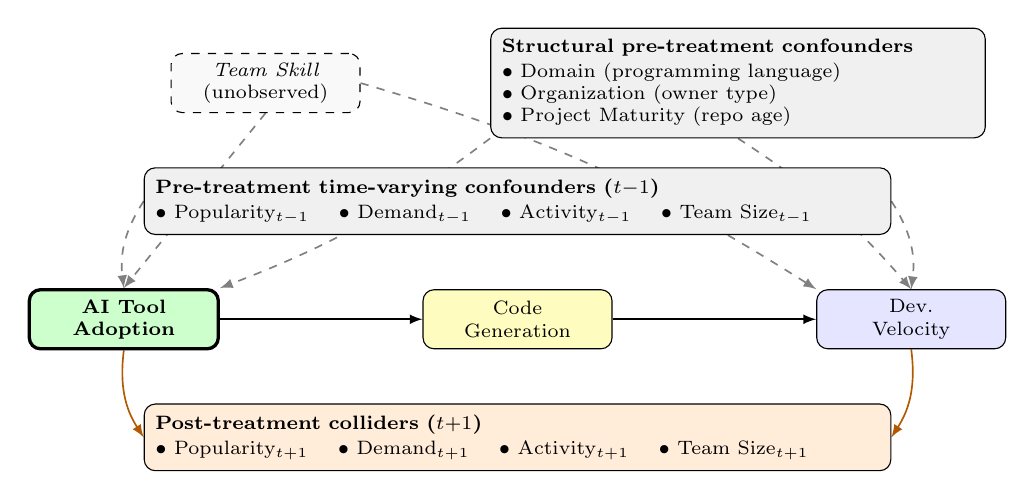
\begin{tikzpicture}[
    >=latex, font=\scriptsize,
    confbox/.style={draw, rounded corners, fill=gray!12, align=left,
                    inner sep=4pt},
    colbox/.style={draw, rounded corners, fill=orange!15, align=left,
                   inner sep=4pt},
    unobs/.style={draw, rounded corners, dashed, fill=gray!5,
                  minimum height=0.75cm, minimum width=2.4cm, align=center,
                  font=\itshape\scriptsize},
    tnode/.style={draw, rounded corners, fill=green!20, very thick,
                  minimum height=0.75cm, minimum width=2.4cm,
                  align=center, font=\bfseries\scriptsize},
    mnode/.style={draw, rounded corners, fill=yellow!25,
                  minimum height=0.75cm, minimum width=2.4cm, align=center},
    ynode/.style={draw, rounded corners, fill=blue!10,
                  minimum height=0.75cm, minimum width=2.4cm, align=center},
    cedge/.style={->, gray, dashed, semithick},
    medge/.style={->, black, semithick},
    coledge/.style={->, orange!70!black, semithick},
]
\pgfdeclarelayer{bg}
\pgfsetlayers{bg,main}
% Row 1: unobserved + structural confounder box
\node[unobs] (skill) at (1.8, 3) {Team Skill\\\emph{(unobserved)}};
\node[confbox, text width=6.0cm] (Struct) at (7.8, 3) {%
    \textbf{Structural pre-treatment confounders}\\[1pt]
    $\bullet$ Domain (programming language)\\
    $\bullet$ Organization (owner type)\\
    $\bullet$ Project Maturity (repo age)
};

% Row 2: pre-treatment time-varying confounder box
\node[confbox, text width=9.2cm] (PreTV) at (5, 1.5) {%
    \textbf{Pre-treatment time-varying confounders ($t{-}1$)}\\[1pt]
    $\bullet$ Popularity$_{t-1}$ \quad $\bullet$ Demand$_{t-1}$ \quad $\bullet$ Activity$_{t-1}$ \quad $\bullet$ Team Size$_{t-1}$
};

% Row 3: causal chain
\node[tnode] (D) at (0, 0) {AI Tool\\Adoption};
\node[mnode] (M) at (5, 0) {Code\\Generation};
\node[ynode] (Y) at (10, 0) {Dev.\\Velocity};

% Row 4: post-treatment collider box
\node[colbox, text width=9.2cm] (PostTV) at (5, -1.5) {%
    \textbf{Post-treatment colliders ($t{+}1$)}\\[1pt]
    $\bullet$ Popularity$_{t+1}$ \quad $\bullet$ Demand$_{t+1}$ \quad $\bullet$ Activity$_{t+1}$ \quad $\bullet$ Team Size$_{t+1}$
};

\begin{pgfonlayer}{bg}
% Back-door edges (dashed gray) -- drawn on background so the PreTV
% confounder box paints on top of the row-1 -> row-3 arrows.
\draw[cedge] (skill.south) -- (D.north);
\draw[cedge] (skill.east) to[bend left=8] (Y.north west);
\draw[cedge] (Struct.south west) to[bend left=8] (D.north east);
\draw[cedge] (Struct.south) to[bend left=8] (Y.north);
\draw[cedge] (PreTV.west) to[bend right=20] (D.north);
\draw[cedge] (PreTV.east) to[bend left=20] (Y.north);

% Causal mechanism (solid black)
\draw[medge] (D) -- (M);
\draw[medge] (M) -- (Y);

% Collider edges (solid orange)
\draw[coledge] (D.south) to[bend right=20] (PostTV.west);
\draw[coledge] (Y.south) to[bend left=20] (PostTV.east);
\end{pgfonlayer}
\end{tikzpicture}
\caption{Temporal DAG for the AI coding tools and development velocity problem, resolving the temporal ambiguity in Figure~\ref{fig:ai-dag} by splitting each time-varying covariate into a pre-treatment node (confounder, gray box) and a post-treatment node (collider, orange box).
Team Skill (dashed border) remains entirely unobserved.
Solid black arrows trace the identified causal path AI Tool Adoption $\to$ Code Generation $\to$ Dev.\ Velocity, dashed gray arrows mark back-door paths from confounders, and solid orange arrows mark edges into the post-treatment colliders.
The back-door criterion yields an unambiguous adjustment set: Condition on all pre-treatment nodes; never condition on post-treatment nodes or the mediator.}
\label{fig:temporal-dag}
\end{figure}

\subsubsection{Temporal Collapse in Cross-Sectional Data}
\label{sec:temporal-collapse}

The temporal DAG makes covariate roles unambiguous---but it requires time-indexed variables.
A typical MSR study queries the GitHub API once at the time of the study, obtaining a single \emph{snapshot} value for each covariate, \emph{collapsing} the time-indexed nodes into a single atemporal variable.
This connects to a recognized problem in the causal inference literature: \citet[Ch.~20]{hernan2020causal} describe this as ``treatment-confounder feedback,'' where time-varying covariates are simultaneously confounders and descendants of treatment.
Table~\ref{tab:covariate-classification} classifies the available covariates by temporal status, in which only three covariates are \emph{structurally pre-treatment} (i.e., determined at creation, under the assumption that changing them along with AI adoption is rare in our studied population): Repository age, primary programming language, and organization ownership.
The remaining covariates are \emph{temporally ambiguous}: Their snapshot values contain both pre-treatment and post-treatment variation, and conditioning on them may introduce collider bias, block causal paths, or both.
In other words, the kitchen-sink regression from snapshot GitHub data does not produce causally interpretable coefficients because of such temporal ambiguity.

\begin{table}[t]
\centering
\caption{Classification of covariates by temporal status.
Only structurally pre-treatment covariates are defensible controls in a cross-sectional analysis; time-varying covariates are temporally ambiguous because their snapshot values mix pre-treatment (confounder) and post-treatment (collider) variation.}
\label{tab:covariate-classification}
\small
\begin{tabular}{lll}
\toprule
Covariate & Temporal Status & Justification \\
\midrule
Repo age & Pre-treatment & Determined at creation \\
Primary language & Pre-treatment & Determined at creation \\
Organization owner & Pre-treatment & Determined at creation \\
\midrule
Stars, Forks & Temporally ambiguous & Accumulate before and after adoption \\
Total commits, PRs, Issues & Temporally ambiguous & Include post-adoption activity \\
Releases & Temporally ambiguous & Include post-adoption releases \\
Repo size (KB) & Temporally ambiguous & Includes post-adoption code growth \\
CI/CD, Wiki, Discussions & Temporally ambiguous & May change as part of adoption wave \\
Open issues & Temporally ambiguous & Snapshot mixes pre/post-adoption state \\
\bottomrule
\end{tabular}
\end{table}

\subsubsection{DAG-Justified Regression}
\label{sec:dag-justified}

Armed with the temporal DAG, we can now construct a principled regression specification.
The temporal DAG in Figure~\ref{fig:temporal-dag} identifies the full adjustment set---all pre-treatment values of time-varying covariates---but the cross-sectional snapshot destroys them.
Thus, we use a longitudinal dataset (Section~\ref{sec:study-setting}) with monthly observations for each repository to recover genuinely pre-treatment values of the time-varying covariates, which include pre-treatment stars, issues, forks, PRs merged, releases, average active contributors, and average monthly commits, for all treated repositories.
This restores the clean temporal structure that the snapshot destroyed and allows us to condition on the full DAG-justified adjustment set---minus Team Skill, which still remains entirely unobserved.

Table~\ref{tab:ols-comparison} compares three OLS specifications: the bivariate regression (no controls), the kitchen-sink model (all snapshot covariates, many temporally ambiguous), and the DAG-justified model (only pre-treatment covariates backed by the temporal DAG).
The bivariate coefficient is $2.314$ ($+911\%$, $R^2 = 21\%$).
The kitchen-sink coefficient attenuates to $0.946$ ($+158\%$, $R^2 = 59\%$) after adding all available controls, but its interpretation is incoherent: The collapsed cross-sectional graph is not a DAG, so no adjustment formula tells us whether we are removing confounding bias, blocking causal paths through mediators, or opening spurious paths through colliders.
The DAG-justified specification further attenuates to $0.696$ ($+101\%$, $R^2 = 83\%$), conditioning only on covariates that the temporal DAG identifies as pre-treatment confounders, each computed from panel data before the treatment month.
This is the only specification with a principled justification from the back-door criterion (Section~\ref{sec:primer-dags}), albeit Team Skill remains an important unobserved confounder.

\begin{table}[t]
\centering
\caption{OLS (ordinary least squares regression) estimates of systematic AI coding tool adoption effect on $\log(\text{monthly commits})$.
The bivariate coefficient reflects raw selection.
The kitchen-sink coefficient adds all snapshot covariates but is uninterpretable because the collapsed graph is cyclic.
The DAG-justified specification conditions only on pre-treatment confounders identified by the temporal DAG (Figure~\ref{fig:temporal-dag}).
All standard errors are heteroscedasticity-robust (HC1)~\cite{mackinnon1985heteroskedasticity}.}
\label{tab:ols-comparison}
\small
\begin{tabular}{lrrrr}
\toprule
Model & Coeff.\ & Robust SE & $p$-value & $R^2$ \\
\midrule
Bivariate (no controls) & 2.314 & 0.124 & ${<}0.001$ & 0.210 \\
Kitchen-sink (all snapshot covariates) & 0.946 & 0.116 & ${<}0.001$ & 0.591 \\
DAG-justified (panel pre-treatment) & 0.696 & 0.090 & ${<}0.001$ & 0.827 \\
\bottomrule
\end{tabular}
\end{table}

\subsubsection{Sensitivity Analysis}
\label{sec:cross-sectional-sensitivity}

The DAG-justified estimate is the most principled cross-sectional specification we can construct, but the temporal DAG reveals an important gap: Team Skill remains entirely unobserved.
No variable in the GitHub API data captures developer expertise, team culture, or organizational practices---the confounders most plausibly responsible for the residual association between AI adoption and development velocity.
Faced with this uncertainty, the researcher can ask: \emph{How robust is the DAG-justified estimate to this unobserved confounding?}

One possible method to probe this question is the proportional selection method of \citet{oster2019unobservable} (Section~\ref{sec:primer-po}).
The intuition is to compare the observed shift in the treatment coefficient that resulted from adding the observable controls with the additional shift an unmeasured confounder would have to produce to drive the coefficient to zero.
If unobservables would need to be \emph{at least as strong as} all the observables combined to eliminate the effect, the result is considered robust to omitted variable bias.
This intuition is captured by the Oster proportional selection statistic $\delta^*$, with the heuristic threshold $\delta^* \geq 1$ marking the robustness boundary.
Moving from the bivariate to the DAG-justified specification, we obtain $\delta^* = 0.12$---far below the threshold of~1.
%Three reinforcing factors drive this fragility:
%\begin{enumerate}[leftmargin=15pt]
%    \item \textbf{Massive coefficient drop.} The treatment coefficient falls from $2.314$ to $0.696$---the observables already explain away 70\% of the na\"ive effect.
%    \item \textbf{High $R^2$.} The DAG-justified model explains 83\% of the outcome variance, leaving little residual room for any additional variable to exploit.
%    \item \textbf{Large $R^2$ jump.} The observables increase $R^2$ from $0.21$ to $0.83$, inflating the denominator of $\delta^*$.
%\end{enumerate}
In other words, given how much the coefficient already dropped and how much variance the observables already explain, even a relatively weak unobserved confounder could eliminate the remaining effect.
In our case, some of the most plausible candidates---developer skill and team culture---are precisely the confounders that no GitHub API data can address, and the impact of these confounders remains unclear.\footnote{SE researchers should be aware that sensitivity analysis for omitted variable bias is itself an active research frontier with no established best practices yet.
The Oster method's $\delta^* \geq 1$ threshold is a widely used heuristic, not a formal test: It assumes omitted variables are uncorrelated with included controls~\cite{diegert2026endogenous} and only measures the strength needed to nullify the coefficient, not to flip its sign~\cite{masten2025sign}.
Alternative approaches---such as the E-value~\cite{vanderweele2017sensitivity} and partial-$R^2$ robustness value~\cite{cinelli2020making}---parameterize confounding strength differently, and each rests on its own assumptions.
No single sensitivity measure is definitive; the pragmatic recommendation is to report multiple measures, state their assumptions transparently, and ultimately rely on domain knowledge to judge whether the unobserved confounders in a given SE setting are plausibly strong enough to alter the conclusions.}

\subsubsection{Comparing Estimators: Regression, PSM, and IPW}
\label{sec:estimator-convergence}

Another common response to the limitations of linear regression is to try a ``better'' estimator that are ``known to be a causal inference method,'' among which two popular methods are propensity score matching (PSM)~\cite{rosenbaum1983central} and inverse probability weighting (IPW)~\cite{horvitz1952generalization}.
The main advantage of these methods is that they reduce dependence on the parametric specification of the outcome model~\cite{ho2007matching}: By balancing the covariate distributions between treatment and control groups through matching or reweighting, they lessen the sensitivity of the estimate to functional-form choices such as linearity.
However, and more importantly, PSM and IPW still belong to the selection-on-observables family~\cite{imbens2009recent}, which shares the same identifying assumption as linear regression: conditional ignorability given the observed pre-treatment covariates.
With the problem is unobserved confounding, all three estimators will still have omitted variable bias that can be arbitrarily large in either direction.
In other words, using PSM or IPW does not automatically make a study ``causal inference,'' and the researcher would still need to argue the plausibility of the identifying assumption through a DAG-encoded causal theory.

\begin{table}[t]
  \centering
  \caption{The estimated effect of systematic AI coding tool adoption on log-transformed monthly commits using the same DAG-justified pre-treatment covariates from three estimators: OLS (ordinary least squares regression), PSM (propensity score matching), and IPW (inverse probability weighting).
  \label{tab:three-estimators}
  All standard errors are heteroscedasticity-robust (HC1)~\cite{mackinnon1985heteroskedasticity}.}
  \begin{threeparttable}
  \small
  \begin{tabular}{lrrrr}
  \toprule
  Method & Coeff.\ & Robust SE & $p$-value & $N$ \\
  \midrule
  OLS (DAG-justified) & 0.696 & 0.090 & ${<}0.001$ & 999\tnote{a} \\
  PSM (1:1 nearest neighbor) & 0.574 & 0.094 & ${<}0.001$ & 456 \\
  IPW (ATT) & 0.509 & 0.091 & ${<}0.001$ & 999\tnote{a} \\
  \bottomrule
  \end{tabular}
  \begin{tablenotes}
  \footnotesize
  \item[a] One repository from the original 1,000 was deleted between the collection of cross-sectional and panel data, reducing the sample to 999.
  \end{tablenotes}
  \end{threeparttable}
  \end{table}

Table~\ref{tab:three-estimators} compares the three estimators using the same DAG-justified pre-treatment covariates, in which OLS gets $\hat{\tau} = 0.696$ (+100.57\%), 1:1 nearest-neighbor propensity score matching gets $\hat{\tau} = 0.574$ (+77.54\%), and ATT-targeted inverse probability weighting gets $\hat{\tau} = 0.509$ (+66.36\%).
The three estimators target slightly different estimands---OLS approximates the ATE while PSM and IPW estimate the ATT---and operate on different effective samples (PSM retains 456 matched observations from the 999 available), which accounts for the variation in effect estimates.
However, if we compare the estimates with the DiD estimates in Section~\ref{sec:did}, it would be reasonable to infer that the OLS, PSM, and IPW estimators are all still inflated because of the unobserved confounders like Team Skill.

\subsubsection{Cross-Sectional Takeaway}
\label{sec:cross-sectional-takeaway}

The cross-sectional analysis illustrates two challenges that empirical SE researchers should be aware of when drawing causal conclusions from cross-sectional snapshot data.
First, cross-sectional designs suffer from \emph{temporal collapse}: The measurement design destroys the temporal ordering that DAGs require, making principled covariate selection difficult for time-varying covariates.
Second, even when panel data are available to recover pre-treatment covariate values, the resulting estimates may be sensitive to unobserved confounding by factors such as developer skill and team culture that no repository-level API data can capture.
Switching to another selection-on-observables estimator such as PSM or IPW does not resolve this limitation, because the bottleneck is the identifying assumption---conditional ignorability given observables---not the choice of estimator.
Despite the limitations, cross-sectional studies remain valuable---and in many settings they are the only feasible design---but researchers should pair them with sensitivity analyses that transparently assess how robust the conclusions are to plausible unobserved confounders.
On the other hand, with longitudinal data, research designs that exploit within-unit variation---comparing the \emph{same} project before and after adoption, thereby absorbing all time-invariant confounders---are particularly powerful and can strengthen identification in the presence of unobserved confounders.
We turn to this approach in Section~\ref{sec:longitudinal}.

\subsection{Longitudinal Methods}
\label{sec:longitudinal}

The cross-sectional analysis in Section~\ref{sec:cross-sectional} revealed an important bottleneck in selection-on-observable methods: \emph{unobserved confounders}, which may be plausible and strong in many empirical SE settings (e.g., team skill, project culture, individual motivation).
One powerful way to address this limitation is to exploit \emph{longitudinal} data and its panel structure.
Specifically, instead of comparing \emph{different} repositories (cross-section), we compare the \emph{same} repository before and after it adopts AI coding tools.
When we look at the same repository over time, every time-invariant characteristic---team skill, project culture, codebase complexity, programming language---is held constant by construction.
This high-level idea motivates longitudinal statistical modeling methods such as the interrupted time series (ITS) analyses and two-way fixed effect (TWFE) models.
More importantly, the limitations of these methods motivates a powerful design-based identification idea (Section~\ref{sec:primer-design}), \emph{difference in differences}.
We will cover all of them in this section.

Our panel consists of 999 repositories observed over 27 months (January 2024 to March 2026), of which 240 adopted AI tools at staggered times (Figure~\ref{fig:treatment-timing}).
We progress through three increasingly credible designs: (1)~a na\"ive before/after comparison, (2)~interrupted time series with repository fixed effects, and (3)~modern difference-in-differences.
Each stage relaxes one strong assumption by introducing a new design element, at the cost of a different, weaker assumption.

\begin{figure}[t]
\centering
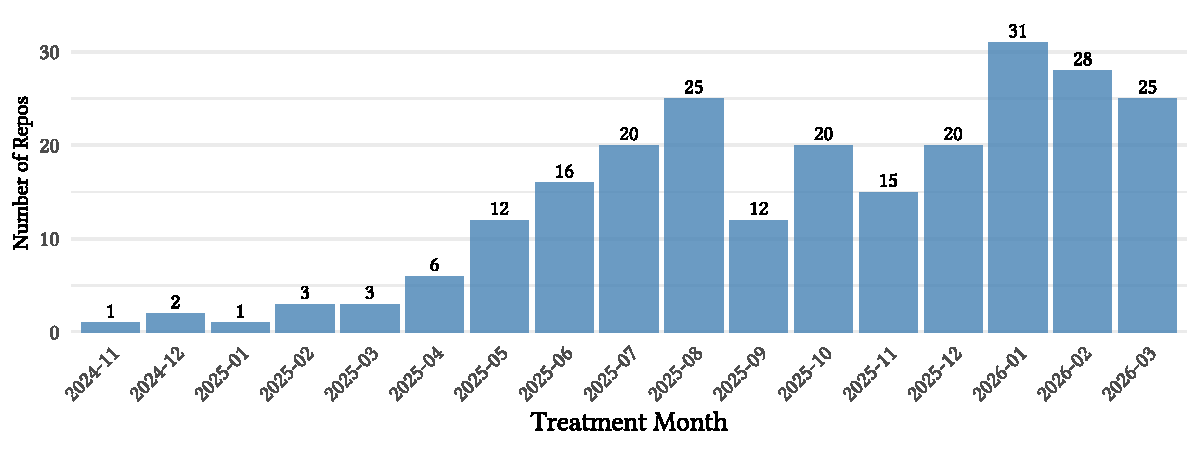
\includegraphics[width=\columnwidth]{figs-tutorial/treatment_timing.pdf}
\caption{Staggered adoption timing.
Each bar shows the number of repositories that first committed an AI configuration file in that month.
The 759 repositories that never adopted during the observation window serve as the control group for the difference-in-differences analysis.}
\label{fig:treatment-timing}
\end{figure}

\subsubsection{Before-and-After Comparison}
\label{sec:before-after}

The simplest within-unit estimator compares, for each treated repository, mean monthly commits (log-scale) before versus after the first AI configuration file commit.
This is the longitudinal analog of the raw group comparison in Section~\ref{sec:naive-comparison}, but now within-unit rather than across units.
A paired $t$-test yields a mean change of $0.940$ (95\% CI $[0.710, 1.180]$), i.e., treated repositories see a 156\% ($\pm$31\%) increase in monthly commits after adoption.
The within-unit pairing absorbs all time-invariant confounders that plagued the cross-section---team skill, project type, organizational practices.
These factors are identical before and after adoption for the same repository, so they cannot drive the observed change.
However, this estimate is causal only if \emph{nothing else} about the treated repositories changed between the pre and post periods, besides the treatment itself.
In other words, the counterfactual outcome---what commits would have looked like without AI adoption---must have stayed flat.
This is a very strong assumption.
If all repositories are growing over 2024--2026 (e.g., due to platform growth, seasonal effects, or the general rise of AI-assisted development), then the before/after estimate captures the treatment effect \emph{plus} the secular trend.
The 156\% figure is almost certainly too high.
This motivates interrupted time series (ITS) analysis that models the trend explicitly.

\subsubsection{Interrupted Time Series (ITS)}
\label{sec:its}

ITS addresses the before/after comparison's key weakness by explicitly modeling the pre-treatment trend.
The regression specification is:
\begin{equation}
\label{eq:its}
Y_{it} = \alpha_i + \beta \cdot t + \delta \cdot \text{Post}_{it} + \gamma \cdot \text{TimeSince}_{it} + \varepsilon_{it}
\end{equation}
where $Y_{it}$ is $\log(1 + \text{monthly commits})$ for repository~$i$ in month~$t$; $\alpha_i$ is a repository fixed effect (one intercept per repository); $\beta \cdot t$ captures the common linear time trend; $\text{Post}_{it}$ equals~1 after adoption and~0 before; and $\text{TimeSince}_{it}$ counts months since adoption (zero before adoption), allowing the slope to change post-treatment.

Each term in Equation~\ref{eq:its} addresses a specific source of confounding.
The repository fixed effects $\alpha_i$ absorb \emph{all} time-invariant unobserved confounders---the exact variables (team skill, project culture, codebase complexity) that made the cross-sectional analysis in Section~\ref{sec:cross-sectional} non-credible.
The time trend $\beta \cdot t$ models a common linear secular trend, so the estimate of $\delta$ is purged of the trend that contaminated the before/after comparison.
ITS thus addresses \emph{two} of the cross-section's core problems simultaneously.
The coefficient $\delta$ tests for a discrete level shift at adoption, while $\gamma$ tests whether the post-treatment growth rate differs from the pre-treatment trend.

\begin{figure}[t]
  \centering
  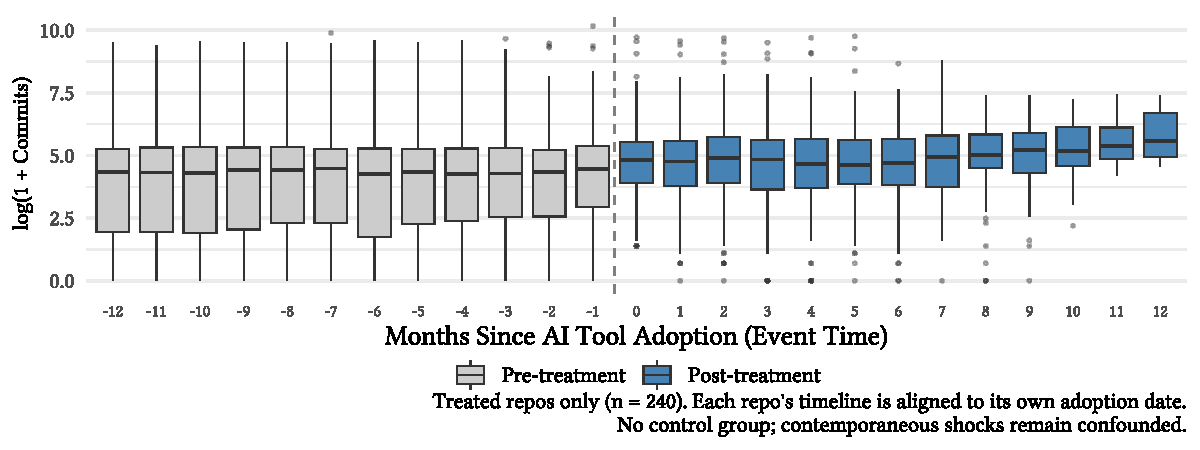
\includegraphics[width=\columnwidth]{figs-tutorial/its_boxplot.pdf}
  \caption{Distribution of $\log(1 + \text{monthly commits})$ by event time for treated repositories.
  Timelines are artificially aligned to each repository's own adoption date.
  ITS models the pre-treatment trend and tests for a level shift at adoption, but lacks a control group to distinguish the treatment effect from contemporaneous shocks.}
  \label{fig:its-boxplot}
\end{figure}

The level-shift estimate is $\hat{\delta} = 0.790$ (95\% CI $[0.550, 1.020]$), i.e., a 120\% ($\pm$26\%) increase.
This is lower than the before/after estimate (156\%), confirming that some of the before/after effect was driven by secular trends that ITS now absorbs.
For $\hat{\delta}$ to have a causal interpretation, the pre-treatment linear trend must be correctly specified, and no other event must systematically coincide with AI adoption.
Unlike the before/after comparison, ITS allows for a secular trend---but it assumes the trend is linear and that the \emph{only} thing that changes at the adoption date is the treatment itself.
Since ITS uses only treated repositories---there is no control group---any shock that happens around the adoption date is indistinguishable from the treatment effect: a team expansion, a major release, a GitHub platform change, or a field-wide shift in development practices.
If such events systematically co-occur with AI adoption, $\hat{\delta}$ absorbs them.
Additionally, if the true pre-treatment dynamics are nonlinear (e.g., accelerating growth from AI or decreasing effectiveness of AI), the linear trend specification may itself be misspecified.

One could address this limitation by adding a control group to the ITS specification---a design known as \emph{controlled interrupted time series} (CITS)~\cite{bernal2017interrupted}---but identification would still depend on correctly specifying the functional form of the trend for both groups.
Difference-in-differences offers a design-based alternative: Rather than modeling the trend explicitly, DiD \emph{differences out} common trends entirely in a natural experiment setting.
The parallel trends assumption (Section~\ref{sec:did}) requires only that treated and control units follow the \emph{same} trend---not that the trend take any particular functional form---making it less demanding than the parametric assumptions underlying ITS and CITS.

\subsubsection{Difference-in-Differences.}
\label{sec:did}

Difference-in-differences (DiD) compares the change in outcomes over time between projects that adopted AI tools and a control group that did not, using the latter group to estimate the trend that the treated projects would have followed absent adoption.
We now add an additional ``control'' group of 759 repositories that never adopted AI tools during the observation window.
An immediate objection arises: The na\"ive comparison in Section~\ref{sec:naive-comparison} showed that adopters and non-adopters differ dramatically in size, activity, and visibility.
How can such different repositories serve as a valid control group?
The answer lies in what DiD actually requires.
Because DiD compares \emph{changes} within each group, all time-invariant differences between groups---no matter how large---cancel out in the differencing.
A small hobbyist project and a large enterprise repository can serve as valid comparisons as long as their commit \emph{trends} would have evolved in parallel absent treatment.
DiD does not require the groups to look alike; it requires them to \emph{trend} alike (see a more formal discussion below).
The key idea is that any time-varying shock that affects both treated and control repositories equally is differenced out, \emph{even without modeling it explicitly}.

In the simplest case (one treatment group, one control group, two periods), the DiD estimator is:
\begin{equation}
\label{eq:did-2x2}
\hat{\tau}^{\text{DiD}} = \bigl(\bar{Y}^{\text{post}}_{\text{treated}} - \bar{Y}^{\text{pre}}_{\text{treated}}\bigr) - \bigl(\bar{Y}^{\text{post}}_{\text{control}} - \bar{Y}^{\text{pre}}_{\text{control}}\bigr)
\end{equation}
The first difference (within each pair of parentheses) removes unit fixed effects---just like the before/after comparison.
The second difference (between the two parentheses) removes common time shocks---exactly what ITS cannot do.
The double difference isolates the treatment effect (which is why it is called \emph{difference in differences}).

The two-way fixed effects (TWFE) regression specification expresses the same idea compactly:
\begin{equation}
\label{eq:twfe}
Y_{it} = \alpha_i + \gamma_t + \tau D_{it} + \varepsilon_{it}
\end{equation}
where $\alpha_i$ is an intercept (or fixed effect term) per repository and absorbs all time-invariant confounders (like ITS), $\gamma_t$ is a intercept per time period and absorbs \emph{common time shocks}, and $\hat{\tau}$ is the DiD estimate.
We present this specification for intuition only and do not report its estimate, for reasons we explain below.

The identifying assumption is \emph{parallel trends}:
\begin{equation}
\label{eq:parallel-trends}
E[Y_{it}(0) - Y_{is}(0) \mid \text{treated}] = E[Y_{it}(0) - Y_{is}(0) \mid \text{control}] \quad \forall\, t, s
\end{equation}
In plain language: absent treatment, treated and control repositories would have followed the same \emph{trend} in outcomes---so matching two groups on levels would be unnecessary if we can show that this assumption is plausible.
Parallel trends is weaker than the ITS assumption: Common shocks are fine as long as they affect both groups similarly.
It is also weaker than the before/after assumption: arbitrary trends are allowed, as long as they are parallel across groups.
We also require a \emph{no-anticipation assumption}: repositories do not change their behavior before they adopt AI tools.

In our setting, repositories adopt at different months, creating a \emph{staggered adoption} design.
Classic TWFE (Equation~\ref{eq:twfe}) implicitly uses already-treated repositories as controls for later-treated ones.
When treatment effects vary across cohorts or over time, this produces negative weights on some group-time ATTs, biasing $\hat{\tau}$~\cite{goodman2021difference, dechaisemartin2020two}.
This well-documented problem (see \citet{roth2023whats} for a survey) motivates modern estimators designed for staggered adoption with heterogeneous effects.
We apply two complementary modern DiD estimators that avoid the negative-weighting problem; Table~\ref{tab:longitudinal-estimators} summarizes the four longitudinal estimators discussed in this section before we detail the two new ones.

\begin{table}[t]
\centering
\caption{Longitudinal estimators discussed in this section, ordered from least to most credible for staggered adoption.
The first two are presented for intuition; the latter two are the modern estimators we actually report.}
\label{tab:longitudinal-estimators}
\footnotesize
\begin{tabularx}{\linewidth}{@{} p{4.0cm} X @{}}
\toprule
\textbf{Estimator} & \textbf{What it does} \\
\midrule
Two-way fixed effects (TWFE)
  & A panel regression with one intercept per unit and one per time period; the simplest DiD specification, but biased under heterogeneous effects with staggered adoption~\cite{goodman2021difference, dechaisemartin2020two}. \\
\addlinespace
Controlled ITS (CITS)~\cite{bernal2017interrupted}
  & Interrupted time series plus a control group; identification still requires correctly specifying the functional form of the pre-treatment trend for both groups. \\
\addlinespace
Callaway \& Sant'Anna (CS)~\cite{callaway2021difference}
  & Estimates a separate ATT per adoption cohort against the never-treated repositories, then aggregates---avoiding the negative-weighting problem of TWFE. \\
\addlinespace
Borusyak et al.\ imputation~\cite{borusyak2024revisiting}
  & Fits a counterfactual model on untreated observations, predicts what the treated repositories' outcomes would have been absent treatment, and averages the residuals as the ATT. \\
\bottomrule
\end{tabularx}
\end{table}

\textbf{Callaway \& Sant'Anna (2021) DiD}~\cite{callaway2021difference} is the most direct extension of the 2$\times$2 idea: it estimates separate treatment effects for each adoption cohort (group of repositories adopting in the same month), then aggregates.
For each cohort $g$ and time period $t$:
\begin{equation}
\label{eq:cs-att-gt}
ATT(g, t) = E[Y_t - Y_{g-1} \mid \text{cohort } g] - E[Y_t - Y_{g-1} \mid \text{never-treated}]
\end{equation}
This is a difference in outcome changes between cohort-$g$ repositories and never-treated repositories, measured from baseline~$g\!-\!1$.
We use no covariates, so this reduces to simple differences in means---the same double-differencing logic as Equation~\ref{eq:did-2x2}, applied separately to each cohort.
The overall ATT averages the group-time effects, weighting by cohort size.
The estimate is $\hat{\tau} = 0.416$ ($\text{SE} = 0.090$), i.e., 52\% ($\pm$14\%).
This unconditional specification relies on parallel trends holding \emph{without} conditioning on covariates.
The CS estimator also allows an alternative specification that conditions on pre-treatment covariates, which we do not report in this chapter because of pre-trend violations.

\textbf{Borusyak et al.\ (2024) imputation DiD}~\cite{borusyak2024revisiting} estimates what outcomes \emph{would have been} without treatment, using a covariate-adjusted counterfactual model, then compares to what actually happened.
The procedure has three steps.
First, it fits a counterfactual model on all untreated observations (never-treated repositories plus pre-treatment periods of treated repositories):
\begin{equation}
\label{eq:borusyak-first-stage}
Y_{it} = \alpha_i + \gamma_t + X_{it}\beta + \varepsilon_{it} \quad \text{for all } (i,t) \text{ with } D_{it} = 0
\end{equation}
This includes time-varying covariates $X_{it}$: $\log$ of contributors, stars, issues, forks, and releases.
Second, for each treated observation, it plugs in the estimated coefficients to predict the counterfactual: $\hat{Y}_{it}(0) = \hat{\alpha}_i + \hat{\gamma}_t + X_{it}\hat{\beta}$.
Third, it computes the ATT as the average residual $\hat{\tau} = \text{mean}(Y_{it} - \hat{Y}_{it}(0))$ across all treated observations, weighting each treated (repository, month) cell equally.
Only untreated observations contribute to the counterfactual model; treated cells are never used as controls for other treated cells, avoiding the negative-weighting problem of TWFE\@.
The estimate is $\hat{\tau} = 0.281$ ($\text{SE} = 0.060$), i.e., 32\% ($\pm$8\%).\footnote{Doubly-robust and machine-learning-based DiD estimators~\cite{santanna2020doubly, chang2020double} further relax the linear functional-form assumption of Equation~\ref{eq:borusyak-first-stage}, but they share the same identifying assumption as Borusyak and would exhibit the same covariate-attenuation mechanism we describe below---the bottleneck is the role of the covariates in the DAG, not the flexibility of the estimator.}

\paragraph{Event Study and Pre-Trends Assessment.}
\label{sec:event-study}
Importantly, both estimators support event-study decompositions that estimate a separate treatment effect $\tau_k$ for each month~$k$ relative to adoption, which can be used to probe whether the parallel trend assumption is plausible (i.e., pre-trend tests).
Specifically, pre-treatment coefficients ($k < 0$) serve as a diagnostic and should be roughly around zero under parallel trends.
Post-treatment coefficients ($k \geq 0$) trace the dynamic treatment effect over time.

\begin{figure}[t]
  \centering
  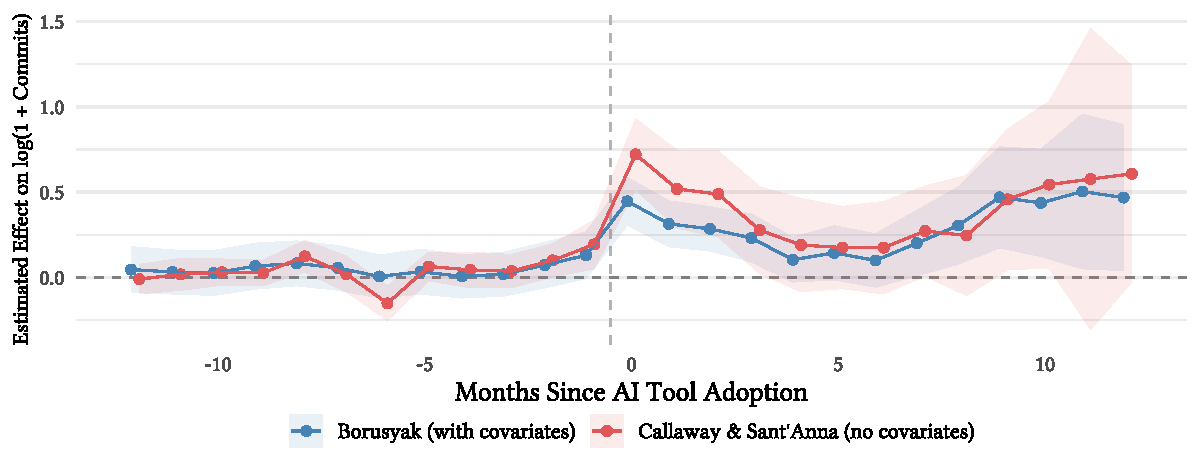
\includegraphics[width=\columnwidth]{figs-tutorial/event_study_comparison.pdf}
  \caption{Combined event study overlaying both DiD estimators.
  Pre-treatment coefficients near zero for both estimators support the parallel trends assumption.
  Post-treatment coefficients show the CS estimate (no covariates) consistently above the Borusyak estimate (with covariates), consistent with the covariate attenuation mechanism discussed in Section~\ref{sec:divergence}.
  Error bars show 95\% confidence intervals.}
  \label{fig:event-study}
  \end{figure}

Figure~\ref{fig:event-study} overlays the event-study estimates from both approaches.
Pre-treatment coefficients cluster near zero for both estimators, supporting the parallel trends assumption.
We assess pre-trends formally with two complementary tests.
For CS, we use simultaneous confidence bands from the \Code{did} package~\cite{callaway2021difference}, which control the family-wise error rate across all pre-treatment periods---a more conservative test than pointwise confidence intervals; 0 of 12 periods are significant under simultaneous bands.
For Borusyak, a joint Wald test pools the 12 pre-treatment coefficients ($H_0\!: \tau_{-12} = \cdots = \tau_{-1} = 0$; $p = 0.70$).\footnote{
It is important to note that passing a pre-trends test does not \emph{prove} parallel trends~\cite{roth2022pretest}.
A more principled alternative is the sensitivity analysis framework of \citet{rambachan2023more}, which asks: How large could post-treatment violations of parallel trends be, relative to any pre-trends we observe, before the conclusion reverses?
This shifts the burden from a binary pass/fail test to a continuous assessment of robustness.
}

\paragraph{Why Does the CS and Borusyak Estimator Diverge?}
\label{sec:divergence}

The primary explanation is \textbf{covariate attenuation}---a direct application of the DAG reasoning from Section~\ref{sec:primer-dags}.
In the imputation step (Equation~\ref{eq:borusyak-first-stage}), the Borusyak model plugs in the \emph{post-treatment} values of the covariates $X_{it}$ to predict the counterfactual $\hat{Y}_{it}(0)$.
If AI adoption causes an increase in contributors or stars---because the tool makes the project more productive and visible---and those in turn drive more commits, then the covariates sit on the \emph{causal pathway}: adoption $\to$ covariates $\to$ commits.
Conditioning on them absorbs part of the treatment's effect, inflating the imputed counterfactual and shrinking the estimated ATT\@.
This is a concrete, numbers-in-hand instance of the mediator bias from Section~\ref{sec:primer-dags}: conditioning on a variable on the causal path between treatment and outcome attenuates the total effect (recall the discussion of colliders and mediators in the temporal DAG, Figure~\ref{fig:temporal-dag}).
The Borusyak estimate of 32\% captures only the effect of AI adoption that does \emph{not} flow through the covariates.
The CS specification omits covariates entirely, so it is unaffected by this mechanism.
Its estimate of 52\% targets the total effect under unconditional parallel trends---but this comes with its own trade-off: if parallel trends holds only \emph{conditional} on covariates, the unconditional estimate may be biased.

A secondary factor is \textbf{aggregation weights}: even without covariate attenuation, the two estimators would differ because they weight heterogeneous cohort-level effects differently---a well-known issue in the recent DiD literature~\cite{roth2023whats}.
Together, the pair of estimates brackets a plausible ATT range of 32--52\%, showing how methodological choices about covariate handling and aggregation can have substantive consequences.

\paragraph{Robustness.}
\label{sec:robustness}

We additionally probe two concerns about control group composition.
First, we trim structurally inactive repositories (fewer than 10 total commits) from the control group, since repositories with flat outcomes may violate parallel trends by failing to track the counterfactual trend of treated repositories.
The Borusyak ATT barely changes ($0.281 \to 0.280$), suggesting the result is not driven by inactive controls.
Second, we restrict the control group to repositories matched on pre-treatment observables via propensity score matching, yielding a similar estimate ($0.301$).
Both checks confirm that the DiD estimates are robust to control group composition.\footnote{Full details of the trimming and matching procedures are available in the replication notebook (Section~\ref{sec:tutorial-data-availability}).}
These robustness checks probe specific threats to internal validity but cannot prove the identifying assumptions; they are best understood as ruling out specific alternative explanations (i.e., inactive controls or uncomparable control groups) as advocated in Section~\ref{sec:primer-stance}.

\paragraph{Longitudinal Takeaway.}
\label{sec:longitudinal-takeaway}

The longitudinal analysis demonstrates the power of design-based identification: by comparing the \emph{same} repository before and after AI adoption, every time-invariant confounder---team skill, project culture, codebase complexity---cancels out by construction, eliminating the single biggest threat to the cross-sectional analysis.
The three-stage progression from before/after (156\%) through ITS (120\%) to DiD (32--52\%) shows that each additional design element---trend modeling, a control group---shrinks the estimate substantially, indicating that secular trends and common shocks inflated the simpler estimates.
Within DiD, the CS--Borusyak comparison (52\% vs.\ 32\%) illustrates a subtle but important lesson: conditioning on post-treatment covariates that lie on the causal pathway attenuates the total effect---an instance of the mediator bias from Section~\ref{sec:primer-dags}.
The remaining threats---parallel trends violations, anticipation effects, and SUTVA violations---are \emph{more transparent and partially testable} (via event studies and pre-trends tests) than the ``all confounders measured'' assumption required by cross-sectional methods.
This transparency is the central advantage of design-based identification.

\paragraph{External Triangulation with Experimental Evidence.}
\label{sec:triangulation}

Beyond methodological defensibility, the DiD estimates gain credibility through comparison with independent experimental evidence on AI coding tools.
The closest construct-matched study is \citet{cui2025effects}, which pools three firm-level field randomized trials ($N = 4{,}867$ developers at Microsoft, Accenture, and a Fortune-100 company) and reports a $+26\%$ increase in completed tasks ($\text{SE} \approx 10\%$).
Shorter-horizon controlled task experiments find larger per-task speedups---\citet{DBLP:journals/corr/abs-2302-06590} report a $55.8\%$ reduction in task-completion time on a single JavaScript task ($N = 95$), and \citet{DBLP:conf/icse-seip/ParadisGMNMMZFC25} report an $\approx 21\%$ time reduction on an enterprise coding task at Google ($N = 96$)---though these measure task speed rather than sustained output volume, so their magnitudes are not directly comparable to monthly commits.
The experimental evidence is not uniformly positive: \citet{DBLP:journals/corr/abs-2507-09089} report a $+19\%$ \emph{slowdown} on 16 experienced maintainers working on 246 issues in mature open-source repositories, and a follow-up with late-2025 data reversed the direction (non-significant speedups of $-4\%$ to $-18\%$) but was flagged by its authors as unreliable due to control-arm attrition~\cite{metr2026uplift}, leaving the effect on experienced open-source maintainers of mature codebases poorly identified as of early 2026.
Our $+32\%$ to $+52\%$ ATT is consistent with the firm-level RCT anchor of \citet{cui2025effects} and sits within the broader range established by these controlled experiments; the na\"ive cross-sectional $+911\%$ is inconsistent with every RCT on record by roughly an order of magnitude.
External triangulation does not validate our DiD estimate in a construct-matched sense---task-time and commit-volume outcomes differ, and open-source and enterprise populations differ---but it shows that the design-based and controlled-experimental evidence agree on the plausible magnitude range, while the na\"ive cross-sectional estimate does not.

\subsection{Summary}
\label{sec:summary}

\begin{table}[t]
\centering
\caption{Summary of all effect estimates from the cross-sectional (Section~\ref{sec:cross-sectional}) and longitudinal (Section~\ref{sec:longitudinal}) analyses.
The estimate is on the $\log(1 + \text{monthly commits})$ scale; the percentage change is $(e^{\text{Estimate}} - 1) \times 100\%$, with $\pm$ computed via the delta method ($e^{\text{Estimate}} \times \text{SE} \times 100\%$).
All OLS specifications approximate the ATE; PSM, IPW, and all longitudinal methods target the ATT.}
\label{tab:all-estimates}
\footnotesize
\setlength{\tabcolsep}{4pt}
\begin{tabularx}{\linewidth}{@{} p{4.6cm} X r r r @{}}
\toprule
Method & Identifying assumption & Estimate & SE & \% change \\
\midrule
\multicolumn{5}{l}{\emph{Cross-sectional (Section~\ref{sec:cross-sectional})}} \\
Na\"ive comparison (no controls) & As-if random assignment & 2.314 & 0.124 & +911\% ($\pm$125\%) \\
Kitchen-sink OLS (snapshot covariates) & Cond.\ ignorability (temporally ambiguous) & 0.946 & 0.116 & +158\% ($\pm$30\%) \\
OLS (DAG-justified, pre-treatment) & Cond.\ ignorability (pre-treatment) & 0.696 & 0.090 & +101\% ($\pm$18\%) \\
PSM (1:1 NN) & Cond.\ ignorability (pre-treatment) & 0.574 & 0.094 & +78\% ($\pm$17\%) \\
IPW (ATT) & Cond.\ ignorability (pre-treatment) & 0.509 & 0.091 & +66\% ($\pm$15\%) \\
\addlinespace
\multicolumn{5}{l}{\emph{Longitudinal (Section~\ref{sec:longitudinal})}} \\
Before/after & Counterfactual outcome stays flat & 0.940 & 0.120 & +156\% ($\pm$31\%) \\
ITS with repo FE & Correct trend; no contemporaneous shocks & 0.790 & 0.120 & +120\% ($\pm$26\%) \\
DiD: CS (no covariates) & Parallel trends (unconditional) & 0.416 & 0.090 & +52\% ($\pm$14\%) \\
DiD: Borusyak (with covariates) & Parallel trends (conditional on $X_{it}$) & 0.281 & 0.060 & +32\% ($\pm$8\%) \\
\bottomrule
\end{tabularx}
\end{table}

Table~\ref{tab:all-estimates} compares all estimates from Sections~\ref{sec:cross-sectional} and~\ref{sec:longitudinal}, along with each method's identifying assumption and its key vulnerability.
It is important to note that the \emph{design} matters more than the estimator.
The na\"ive comparison ($+911\%$) drops to $+158\%$ once we add snapshot controls, and further to $+101\%$ once we condition only on pre-treatment confounders justified by the temporal DAG---each step removes a different source of bias.
Yet within the DAG-justified cross-section, switching from OLS to PSM to IPW still yields estimates higher than the DiD estimates: All three share the conditional ignorability assumption which is violated by the unobserved confounders that no GitHub API data can capture.
Across longitudinal designs, the estimates change dramatically: the before/after estimate (156\%) drops to 120\% with ITS (which absorbs secular trends) and further to 32--52\% with DiD (which absorbs common shocks via a control group).
Each step trades a strong assumption for a weaker one, and the estimates shrink accordingly.
The identifying assumption is progressively weaker and more plausible as we move from the cross-sectional to the longitudinal designs.
The design-based estimates are not only methodologically defensible; they are also the only estimates in Table~\ref{tab:all-estimates} consistent with the magnitude range reported by field experiments on AI coding tools (Section~\ref{sec:triangulation}).

\section{Discussion}
\label{sec:discussion}

This tutorial argued that the SE community should adopt the modern causal inference toolkit as the standard for intervention-outcome questions involving observational data.
We now reflect on what the worked example reveals about current practice, discuss implications for different audiences, and acknowledge limitations and open frontiers.

\subsection{Lessons from the Worked Example}

The progression of estimates in Table~\ref{tab:all-estimates} is the chapter's most concrete argument for why identification strategy matters.
The na\"ive cross-sectional comparison yields $+911\%$; adding snapshot controls reduces this to $+158\%$; conditioning only on DAG-justified pre-treatment covariates further reduces it to $+101\%$; and the staggered DiD estimates land at $+32\%$ to $+52\%$.
Each step removes a specific, named source of bias---temporal ambiguity, collider conditioning, time-invariant confounding, secular trends, common shocks---and each reduction is substantial.
The design, not the estimator, drives the change: Within the cross-sectional family, switching from OLS to PSM to IPW may improve the estimate but they are all plagued by the same conditional ignorability assumption---that all confounders are measured and adjusted for---which is violated whenever an unobserved confounder remains.
The magnitude of this shrinkage matters beyond methodological tidiness.
For many intervention-appraisal questions---how to allocate resources, whether to invest in a technology, whether to adopt a practice---the decision-relevant quantity is \emph{how much}, not merely the direction of the effect~\cite{lundberg2021estimand}, and an order-of-magnitude-inflated estimate can lead to qualitatively different conclusions even when the sign is preserved.

This pattern is unlikely to be unique to our setting.
Many MSR studies query the GitHub API once, obtain a cross-sectional snapshot, regress an outcome on a treatment indicator with available controls, and report the surviving coefficient as suggestive of an effect.
The temporal DAG analysis (Section~\ref{sec:temporal-collapse}) revealed that this workflow destroys the temporal ordering required for principled covariate selection: Variables that are confounders in their pre-treatment incarnation become colliders in their post-treatment incarnation, and a single snapshot conflates the two.
A practical recommendation follows: MSR researchers should invest in constructing longitudinal datasets---mining git histories, leveraging GHArchive time series, recording adoption timing---rather than relying on atemporal snapshots.
The marginal cost of building a panel is modest; the marginal gain in identification is large.

The worked example also produces a substantive finding.
Under the staggered DiD design, systematic AI coding tool adoption---as signaled by AI configuration files committed to the repository---is associated with a 32--52\% increase in monthly commits (the ATT, i.e., the average effect among the adopting projects).
This estimates the effect of the \emph{entire bundle}: The AI tools themselves, the workflow reorganization that accompanies structured adoption, and the team characteristics that lead to early integration (Section~\ref{sec:study-setting}).
It does not isolate the effect of AI code generation alone.
Pre-treatment trend tests support the parallel trends assumption, but the estimate is likely conservative due to control-group contamination: Individual developers using AI tools without project-level configuration files are unobservable, blurring the treated--control contrast and attenuating the estimate toward zero.
We offer this as a credible first estimate that future work can refine with richer treatment definitions, complementary identification strategies, or alternative outcome measures.
The $+32\%$ to $+52\%$ range is also consistent with the field-experimental evidence base on AI coding tools (Section~\ref{sec:triangulation}), most directly with the $+26\%$ pooled estimate from the three firm-level randomized trials in \citet{cui2025effects}, and sits above the null-to-slowdown findings of \citet{DBLP:journals/corr/abs-2507-09089} on experienced maintainers of mature open-source repositories.
The na\"ive cross-sectional $+911\%$ is inconsistent with every published RCT by roughly an order of magnitude, illustrating that the design-based estimates are not only methodologically defensible but also the only estimates in this chapter that triangulate with independent experimental evidence.

\subsection{Implications}

\paragraph{For Reviewers and Editors.}
When a paper poses an intervention-outcome research question, reviewers should require an explicit discussion of the extent to which the evidence supports a causal claim and the assumptions under which it does so.
A regression coefficient presented as ``the effect of $X$ on $Y$'' without an identification argument is not a causal finding---it is a descriptive association whose causal content is unknown.
The empirical standard in Appendix~\ref{sec:appendix-standard} provides a concrete checklist: Does the study state its causal question? Articulate a target trial? Define the estimand? Name the identification strategy and its assumptions? Conduct sensitivity analysis? Engage with alternative explanations?
We encourage editorial boards of SE venues to formally adopt this standard---or one like it---into the ACM SIGSOFT Empirical Standards collection, following the precedent of editor-endorsed guidance in respiratory and critical care medicine~\cite{lederer2019control} and emerging norms in psychology~\cite{grosz2020taboo} and epidemiology~\cite{hernan2018cword}.
This does not mean that every empirical SE paper must become a causal study; descriptive, predictive, and qualitative studies remain indispensable.
The standard applies specifically when a study asks a causal question, and a lot more empirical SE papers can possibly reframe their research question to be causal, as many of them already have a causal motivation in mind (see Section~\ref{sec:bg-adoption}).

\paragraph{For Researchers.}
The causal inference toolkit can seem daunting, but the barrier to entry is lower than it appears.
The pragmatic stance in Section~\ref{sec:guide} provides a workflow; the FAQ in Appendix~\ref{sec:appendix-faq} addresses common objections and recommends software tools; and a new generation of accessible textbooks~\cite{cunningham2021causal, huntingtonklein2021effect, hernan2020causal, angrist2009mostly} makes self-study feasible.
The most important first step is not mastering a specific method but adopting a way of thinking: Before fitting a model, articulate the target trial, sketch a DAG, ask what variation in the data identifies the causal effect, and reason whether the identification assumption would be plausible in the specific study setting.
This exercise alone---even without changing the statistical method---often reveals problems invisible to the standard regression workflow: a key covariate is a mediator, the treatment is poorly defined, or the research question conflates two distinct estimands.
Causal inquiry is inherently iterative: The first identification strategy will have gaps, and revision is the norm, not the exception.

\subsection{SE's Advantages for Causal Inference}

Our message is not that SE is behind---it is that SE has untapped potential.
Several structural features of SE data make it unusually well suited to the design-based methods this tutorial advocates.
First, SE data is inherently \emph{panel data}: Repositories have commit histories spanning years, developers contribute across projects over time, and tools and practices are adopted in staggered fashion---precisely the structure that DiD, panel fixed effects, and synthetic control designs exploit.
Second, SE has the data infrastructure---version control systems, public repositories, platform event streams---that researchers in economics, psychology, or epidemiology often cannot access.
Finally, SE ecosystems generate rich \emph{quasi-experimental variation}: Platform policies (GitHub Actions rollout, npm security mandates, language deprecation announcements), organizational mandates, and ecosystem-wide shocks create exogenous variation that resembles natural experiments.
The field is rich in settings where design-based identification is feasible; it has simply not been exploited at scale.

The causal inference framework also creates a productive bridge between qualitative and quantitative SE research.
Every step of a causal inquiry---framing the question, proposing a DAG, choosing covariates, interpreting results---requires \emph{domain knowledge} that cannot be derived from data alone (Section~\ref{sec:stance-prior-research}).
Interviews, case studies, practitioner postmortems, and gray literature become the theory-generating engine that proposes causal structures; rigorous quantitative designs then test them; and the findings refine theory for the next iteration.
Far from marginalizing qualitative research, the toolkit makes its role in theory-building explicit and essential.

\subsection{Limitations and Open Frontiers}

Raising empirical standards cannot prevent the superficial or ritualistic adoption of methods---applying DiD without understanding parallel trends, or drawing a DAG without genuine engagement with the causal structure.
This concern is not hypothetical: The SE community has experienced analogous problems with the adoption of qualitative methods, where the label is adopted but the disciplined reasoning behind the method is not~\cite{DBLP:journals/tosem/RobillardAEGLNNSSS24}.
The antidote is peer review informed by the empirical standard (Appendix~\ref{sec:appendix-standard}) and a culture of substantive engagement with identification assumptions---evaluating whether a study's parallel trends argument is plausible, not merely whether the words ``parallel trends'' appear.

Several SE-specific challenges deserve particular attention as open research frontiers.
First, SE treatments are often \emph{compound}: ``Adopting AI coding tools'' bundles the tools themselves, the workflow reorganization, and the team characteristics that drive adoption (Section~\ref{sec:study-setting}).
Developing decomposition strategies for disentangling bundled interventions in SE settings is an important methodological direction.
Second, interconnected software ecosystems create \emph{SUTVA violations}---i.e., one project's treatment status affects another project's outcomes, breaking the no-interference assumption that standard estimators rely on: Shared libraries propagate effects across projects, developer mobility carries practices between teams, and upstream changes spill over into downstream dependencies.
Adapting causal inference methods under network interference~\cite{savje2021average, forastiere2021identification} to SE's sociotechnical dependency structures is an open frontier where SE-specific methodological contributions could flow back to the broader causal inference community.
Third, our worked example reports a single ATT, but the effect of AI coding tools is almost certainly \emph{heterogeneous}---varying across programming languages, team sizes, project maturity, and adoption cohorts.
Machine-learning estimators for conditional average treatment effects---which estimate how the treatment effect varies with covariates rather than reporting a single average---such as causal forests~\cite{wager2018estimation} and double/debiased machine learning~\cite{chernozhukov2018double}, offer tools for characterizing this heterogeneity, but they inherit the identifying assumptions of simpler estimators and are therefore most useful once identification has been established.
Systematically mapping effect heterogeneity in SE settings---where treatment effects may interact with ecosystem position, developer experience, or project governance structures---is a natural next step for studies that have cleared the identification bar.
Finally, even as the community improves identification, corresponding investment in measurement validity---construct definition, proxy validation, and triangulation across multiple outcome measures~\cite{lawlor2016triangulation}---is essential.
A perfectly identified design with a bad outcome proxy still produces misleading conclusions.
Identification and measurement are orthogonal challenges (Section~\ref{sec:primer-stance}); this tutorial addresses the former, but the latter demands equal attention.

\section{Conclusion}

No single observational study resolves a causal question definitively.
The field builds general causal knowledge through \emph{triangulation}: accumulating credible local estimates across complementary designs, data sources, and populations~\cite{shadish2002experimental}---just as economics built its evidence base on minimum wage effects and returns to education through dozens of independent, credible studies that converged~\cite{angrist2010credibility}.
SE's diversity of ecosystems---different languages, platforms, team structures, development cultures---makes it well suited to this strategy: The same causal question can be studied in many independent settings, each with its own identification strategy, and convergence across them is far more persuasive than any single study claiming a universal effect.

The causal inference toolkit's greatest contribution to SE is not a specific method but a way of thinking: making identifying assumptions \emph{transparent and open to scrutiny} so that the strength of evidence is clearly communicated and the field can iteratively develop stronger designs.
We envision this adoption bringing productive advancements on a broad range of important intervention-outcome questions---from the effect of AI coding tools to the impact of development practices, governance structures, and ecosystem policies---moving the field from the blanket disclaimer that ``correlation does not imply causation'' toward the constructive discipline of asking: \emph{Under what assumptions does this evidence support a causal interpretation, and how can the next study relax those assumptions?}

The three empirical chapters that follow put this way of thinking into practice.
Each applies the four-step causal credibility assessment introduced in Section~\ref{sec:thesis-statement} to a widely held software engineering myth, stating the causal theory, the estimand, and the identifying assumptions explicitly so that the reader can judge under what conditions the myth holds.

\section{Data Availability}
\label{sec:tutorial-data-availability}

All data, analysis scripts, classification prompts, and R~notebooks used in this chapter are publicly available at \url{https://github.com/hehao98/CausalityInSE}.
The repository includes the LLM-classified corpus of 5,341 SE papers (Section~\ref{sec:bg-adoption}), the AI adoption dataset of 1,000 GitHub repositories with monthly commit histories (Section~\ref{sec:worked-example}), and all R~Markdown notebooks that reproduce the figures, tables, and statistical analyses reported in this chapter.

\section{Appendix}

% The tutorial's appendix is written with \section/\subsection headings.
% Demote them one level so they nest under this chapter-level appendix section.
\let\origsection\section
\let\origsubsection\subsection
\let\section\subsection
\let\subsection\subsubsection

\section{The Causal Inference Toolkit: Historical Development and Parallels with Other Disciplines}
\label{sec:appendix-history}

This appendix provides a detailed account of the intellectual traditions that produced the causal inference toolkit introduced in Section~\ref{sec:bg-causal-history}, followed by a summary of methodological reforms in psychology and epidemiology in which they recently started to address causal inference problems similar to those we identify in SE\@.

\subsection{The Development of the Causal Inference Toolkit}
\label{sec:appendix-toolkit-history}

The modern causal inference toolkit emerged over a century through contributions from three intellectual traditions---statistics, econometrics, and computer science---each addressing a distinct aspect of causal inference: experimental foundations, credibility evolution, and graphical modeling.

First, statisticians laid the \emph{experimental foundations}.
\citet{neyman1923application} defined the causal effect as the difference between two potential outcomes---only one of which is ever observed---and \citet{fisher1935design} established randomization as the principled basis for causal attribution.
Extending causal reasoning to observational settings, \citet{hill1965environment} proposed viewpoints for evaluating whether observed associations reflect genuine causal relationships, \citet{rubin1974estimating} formalized \emph{conditional ignorability} as the identifying assumption for observational studies, and \citet{rosenbaum1983central} introduced the propensity score as a practical dimension-reducing device for covariate adjustment.
Yet, the family of selection-on-observables methods fundamentally cannot address confounding from \emph{unobserved variables} plaguing many economic and societal problems~\cite{heckman1979sample}---e.g., one's (arguably unmeasurable) inherent ability affects both their educational attainment and future earnings~\cite{card1999causal}---a limitation that motivated economists to develop design-based alternatives.

Then, econometricians drove the \emph{credibility revolution}, shifting the basis of causal claims from statistical modeling to research design.
\citet{leamer1983let} first diagnosed the field's credibility problem, arguing that the sensitivity of regression results to specification choices undermined confidence in empirical findings.
The constructive response came through landmark natural experiments: \citeauthor{card1994minimum}'s~\cite{card1994minimum} difference-in-differences analysis of a minimum wage increase demonstrated that design-based evidence can overturn decades of cross-sectional conventional wisdom, and \citet{angrist1996identification} formalized instrumental variable identification through the LATE theorem.
\citet{angrist2010credibility} crystallized the overarching manifesto: Design-based studies yield more credible causal evidence than advances in statistical modeling alone.
The 2021 Nobel Memorial Prize in Economic Sciences, awarded to Card, Angrist, and Imbens for \emph{``their methodological contributions to the analysis of causal relationships''}~\cite{nobelprize2021economics}, cemented the credibility revolution as one of the most consequential intellectual movements in modern social science research.

From computer science and artificial intelligence (specifically the line of research on Bayesian networks and probabilistic reasoning~\cite{pearl1988probabilistic}), \citet{pearl2009causality} developed the graphical causal model framework, representing causal relationships as directed acyclic graphs (DAGs) and introducing the \emph{do-calculus} and \emph{back-door criterion} for determining sufficient adjustment sets.
Where the potential outcomes tradition defines \emph{what} to estimate, DAGs provide a visual language for arguing \emph{why} identification assumptions hold.
\citet{morgan2015counterfactuals} bridged the two traditions for social science, and \citet{imbens2020potential} clarified their relative strengths, arguing that potential outcomes are more natural for design-based research while DAGs excel at encoding complex causal structures.

Recent cross-disciplinary advances have extended the toolkit further: double/debiased machine learning for high-dimensional settings~\cite{chernozhukov2018double}, causal forests for heterogeneous effects~\cite{athey2016recursive}, modern DiD estimators robust to staggered adoption~\cite{callaway2021difference, roth2023whats}, and sensitivity analysis tools for assessing vulnerability to unobserved confounding~\cite{rosenbaum2002observational, oster2019unobservable, cinelli2020making}.
A new generation of accessible textbooks~\cite{angrist2009mostly, hernan2020causal, cunningham2021causal, huntingtonklein2021effect} has demonstrated that these methods can be taught to non-specialist audiences; \citeauthor{hernan2020causal}'s~\cite{hernan2020causal} \emph{target trial} framework, which asks researchers to describe the hypothetical randomized trial their observational analysis attempts to emulate, is particularly relevant to SE\@.
Our tutorial treats both traditions as essential for SE research: Design-based identification provides credible effect estimates for SE interventions while graphical causal models help the decomposition of mechanisms in which the intervention affects the outcome---both are critical for a full understanding of empirical SE problems (Section~\ref{sec:primer}).


\subsection{The Methodological Reform in Psychology and Epidemiology}
\label{sec:appendix-psych-reform}

In recent years, psychology and health research have confronted a causal inference problem similar to what we identify in SE---the disconnect between causal ambition and methodological practice---and their experience reveals both consequences and remedies relevant to the SE community.

The reform began with the diagnosis of the causal language problem.
\citet{hernan2018cword} challenged the epidemiological norm of replacing causal language with associational euphemisms, arguing that this evasion does not prevent causal interpretation but merely obscures the causal question and blocks transparent discussion of identification assumptions.
\citet{grosz2020taboo} documented a parallel ``taboo'' in psychology: The norm against explicit causal inference pushes causal reasoning underground, resulting in impaired study design and a disconnect between findings and downstream interpretation.
\citet{haber2022causal} provided large-scale empirical evidence that this taboo fails on its own terms---among 1,170 articles from 18 high-profile health journals, 52\% of abstracts implied moderate or strong causality despite ostensibly associational language.
The SE community exhibits the same pattern, as we will show in Section~\ref{sec:bg-adoption}.

In response, methodological reformers borrowed tools from the causal inference traditions described above.
\citet{rohrer2018thinking} introduced DAGs to psychology, and \citet{wysocki2022statistical} demonstrated that controlling for mediators, colliders, or their descendants can introduce \emph{more} bias---a finding directly applicable to SE studies that include covariates without causal justification.
\citet{lundberg2021estimand} formalized the \emph{estimand-first} principle for sociology, requiring every study to define its target quantity outside any particular statistical model.
Institutionally, \citet{lederer2019control} issued editor-endorsed guidance requiring authors to specify causal questions and justify covariate selection---editorial policy that does not yet exist in any SE venue.
\citet{tennant2021dags} assessed DAG adoption in health research and found that only 21\% of articles reported target estimands, revealing a theory-practice gap that parallels \citeauthor{DBLP:journals/infsof/Siebert23}'s~\cite{DBLP:journals/infsof/Siebert23} findings in SE\@.

High-profile case studies have illustrated the consequences of ignoring causal reasoning.
\citet{killingsworth2023income} appeared to resolve the long-standing income--happiness debate through sophisticated observational analysis, only for \citet{rohrer2024inappropriate} to demonstrate that the resolution rested on untested identification assumptions---effectively performing the causal assessment our framework codifies.
This sequence mirrors the trajectory from \citet{DBLP:conf/sigsoft/RayPFD14} through \citeauthor{DBLP:journals/toplas/BergerHMVV19}'s~\cite{DBLP:journals/toplas/BergerHMVV19} in SE: In both cases, increasingly sophisticated correlational analyses cannot resolve causal questions without explicit identification.
\citeauthor{rohrer2024causal}'s~\cite{rohrer2024causal} recent tutorial for psychologists is the closest existing analog to our work but does not cover design-based identification strategies or SE-specific confounding structures.
The solutions emerging across these disciplines---explicit causal questions, DAG-based covariate justification, estimand-first workflows, sensitivity analysis, and editorial enforcement---can inform and accelerate SE's own methodological reform.


\section{Frequently Asked Questions}
\label{sec:appendix-faq}

% ---------------------------------------------------------------------------
% Category 1: Foundational and Philosophical
% ---------------------------------------------------------------------------

\subsection{A complete causal model of a sociotechnical system might require thousands of variables. Does that mean causal inference is hopeless without a complete theory?}

No.
Science has never required complete theories, and causal inference is no exception.
The back-door criterion (Section~\ref{sec:primer-dags}) requires blocking all \emph{back-door paths} between treatment and outcome---not enumerating every variable in the universe.
A DAG with eight well-chosen nodes can achieve identification that a regression with two hundred covariates cannot, because what matters is whether the adjustment set blocks every confounding path, not how many variables appear in the model.
Moreover, sensitivity analysis methods allow researchers to quantify how strong an unmeasured confounder would need to be to overturn a finding~\citep{vanderweele2017sensitivity, oster2019unobservable} so that a study can provide credible evidence even without a complete causal model.
Meanwhile, design-based methods (Section~\ref{sec:primer-design}) sidestep the completeness problem entirely.
Difference-in-differences, panel fixed effects, and instrumental variables derive identification from features of the research setting---temporal variation, staggered adoption, quasi-random assignment---rather than from a claim that all confounders have been measured.
These methods require their own assumptions, but those assumptions concern the \emph{specific variation exploited}, not the completeness of the researcher's world model.

The broader philosophical stance is this: Every empirical study embeds causal assumptions, whether the researcher states them or not.
A regression that ``controls for'' five variables implicitly assumes that those five variables suffice to block all confounding---an assumption that is invisible, unexamined, and typically unjustified.
Causal inference does not demand that assumptions be \emph{correct}; it demands that they be \emph{transparent}.
Partial, explicit causal reasoning is strictly better than implicit, unexamined causal assumptions hiding inside every regression coefficient.

\subsection{My regression has $R^2 = 0.99$. Have I controlled for all confounders?}

No.
$R^2$ measures \emph{predictive} fit---how much variance in the outcome the model explains---not causal identification.
These two properties are logically independent, and conflating them is a common source of false confidence.

For example, suppose we want to estimate the effect of adopting code review ($T$) on post-release defect count ($Y$), and the true causal effect is $\beta_T = -5$ defects.
Developer inexperience ($U$) is an unmeasured confounder: Teams mandate code review for junior developers, and those same developers independently produce more defects.
We include lines of code (LOC) as a control variable, which is one of the strongest known predictors of defect counts in the empirical SE literature~\cite{DBLP:journals/tse/GravesKMS00, DBLP:journals/tse/EmamBGR01, DBLP:books/oreilly/11/HerraizH11}.
Regressing $Y$ on $T$ and LOC yields $R^2 \approx 0.99$ because LOC absorbs nearly all variance in defect counts.
But this near-perfect fit is causally misleading.
If LOC is a \emph{mediator}---code review encourages cleaner and smaller codebase that would have fewer defects---then conditioning on it blocks the indirect causal path $T \to \text{LOC} \to Y$, absorbing part of the genuine treatment effect into LOC's coefficient.
Meanwhile, the back-door path through $U$ remains wide open.
Because inexperienced developers both receive mandatory review ($U \to T$) and produce more defects ($U \to Y$), the unmeasured confounder induces a \emph{positive} spurious association between $T$ and $Y$---an upward bias.
Conditioning on LOC absorbs the genuine indirect effect while leaving this confounding bias intact.
If the confounding is strong enough, it can even \emph{flip the sign}.
A regression on $T$ and LOC may yield $\hat{\beta}_T \approx +1$, suggesting that code review \emph{increases} defects, when the true causal effect is $\beta_T = -5$.
The $R^2$ remains $0.99$ throughout, offering no warning that the coefficient is not merely biased but directionally wrong.
Had we instead omitted LOC and used a design-based strategy to address $U$, the model's $R^2$ might be a modest $0.35$---yet the causal estimate would be unbiased.

More generally, a model can achieve near-perfect $R^2$ while producing severely biased causal estimates.
This happens when the model includes \emph{mediators}---variables on the causal path from treatment to outcome---which block the genuine effect the researcher seeks to detect (Section~\ref{sec:primer-naive}).
It also happens when the model includes \emph{colliders}---common effects of treatment and outcome---which open spurious paths rather than closing them.
In both cases, $R^2$ rises because the added variable explains outcome variance, but the treatment coefficient moves \emph{away} from the true causal effect.
Conversely, a correctly specified causal model may have low $R^2$ because many factors affect the outcome but are unrelated to the treatment---the causal estimate can be unbiased even when the model explains little overall variance.

\subsection{I have a multivariate regression with 1000 covariates measuring everything I can think of in the study setting. Does that mean that I have sufficiently controlled for the important confounders?}

No---and in many cases, adding variables \emph{increases} bias.
This counterintuitive result follows directly from the causal structure of the data-generating process, which may make adding a variable introduce \emph{mediator bias} and \emph{collider bias} while not addressing unobserved confounders (see Section~\ref{sec:primer-naive} and Section~\ref{sec:primer-dags}).
Consequently, ``throwing in everything available'' is not a conservative strategy---it is a gamble whose expected payoff depends on the causal structure, which regression alone cannot reveal~\cite{wysocki2022statistical}.
The back-door criterion provides the principled alternative: Include variables that block confounding paths; exclude mediators, colliders, and their descendants.

\subsection{What is the role of DAGs in selection-on-observables vs.\ design-based identification?}

The two identification families use DAGs differently, and understanding this distinction clarifies what each requires from the researcher.
In \emph{selection-on-observables} methods---regression, matching, inverse probability weighting---DAGs are \emph{essential}.
The back-door criterion (Section~\ref{sec:primer-dags}) is the only principled basis for deciding which covariates to include and which to exclude.
Without a DAG, the researcher has no formal basis for determining whether the covariate set blocks all confounding paths, and covariate selection defaults to convenience, tradition, or data availability---none of which bear any necessary relationship to causal identification.
In \emph{design-based identification}---difference-in-differences, instrumental variables, regression discontinuity, panel fixed effects---DAGs play a \emph{supporting} role.
The design itself provides identification through quasi-random variation, so the researcher does not need a complete DAG to determine the adjustment set.
However, a partial DAG remains valuable for three purposes: clarifying which confounders the design absorbs (e.g., panel FE absorbs all time-invariant confounders), assessing whether design-specific assumptions are plausible (e.g., whether the exclusion restriction for IV holds, or whether unmeasured time-varying confounders threaten panel FE), and reasoning about the mechanisms through which the treatment affects the outcome.
One who draws even a partial DAG reasons more clearly about what their design does and does not address.
Both identification families benefit from making assumptions visual and debatable~\cite{imbens2020potential}.

% ---------------------------------------------------------------------------
% Category 2: "My Current Methods Work Fine"
% ---------------------------------------------------------------------------

\subsection{I already control for confounders in my regressions and report threats to validity. What does causal inference add?}

Two things: discipline and tools:
\begin{enumerate}[leftmargin=15pt]
    \item \emph{Discipline}:
    Causal inference forces the researcher to define the estimand before choosing a method (Section~\ref{sec:primer-stance}), construct a DAG that makes every assumption explicit, and justify each covariate on causal---not statistical---grounds.
    This discipline routinely reveals problems invisible to the standard regression workflow: The study answers a different question than intended (e.g., ATT when the research question concerns ATE), a key covariate is a mediator whose inclusion blocks the effect of interest, or a ``control variable'' is a collider whose inclusion opens a spurious path.
    The estimand-first principle~\cite{lundberg2021estimand} ensures that the statistical procedure is evaluated against a well-defined target quantity, not assessed only on internal statistical criteria.
    \item \emph{Tools}:
    Design-based methods---difference-in-differences, panel fixed effects, instrumental variables---can absorb entire categories of unmeasured confounders that no regression can adjust for (Section~\ref{sec:primer-design}).
    Panel fixed effects, for example, remove \emph{all} time-invariant confounders---developer experience, team culture, organizational practices---without requiring them to be measured.
    These methods are strictly more powerful than covariate adjustment in settings where SE data has the temporal or panel structure that design-based identification exploits.
\end{enumerate}

\subsection{What is wrong with interpreting regression coefficients as causal effects?}

A regression coefficient has a causal interpretation \emph{only} when specific identifying assumptions are satisfied: conditional ignorability (all confounders measured), correct functional form, and no conditioning on mediators or colliders (Section~\ref{sec:primer-po}).
Without explicitly stating and defending these assumptions, the coefficient is a descriptive association whose causal content is unknown.
If a researcher simply fits a regression, reports coefficients, and interprets it in causal language in the discussion, this is exactly the pattern that the ``Table~2 fallacy''~\cite{westreich2013table2} describes.
Being careful about modeling choices (variable selection, outlier treatment, functional form) is necessary but not sufficient: It addresses statistical concerns while leaving the causal identification question unanswered.
A well-specified regression with all the right controls is a valid identification strategy---but the researcher must \emph{argue} that the controls are right, using a DAG or substantive domain knowledge, not hope that statistical diligence substitutes for causal reasoning.

\subsection{I run controlled experiments with developers. Why do I need observational causal inference methods?}

Controlled experiments are the gold standard for internal validity and nothing in this tutorial diminishes their value.
But many of the most important SE questions---Does adopting a language reduce defects in production?
Does code review improve long-term maintainability?
Does CI/CD adoption increase deployment frequency?---cannot be answered with lab experiments because they involve organizational decisions, long time horizons, and populations that cannot be randomly assigned.
Observational causal inference methods are designed precisely for these settings.

The target trial framework (Section~\ref{sec:primer-causality}) bridges the two worlds: It asks the researcher to describe the experiment they wish they could run and then evaluates how far their observational design departs from that ideal.
SE researchers who are already comfortable with controlled experiments~\cite{DBLP:books/sp/WohlinRHORW24} will find this framing natural---it simply extends the experimental logic to settings where randomization is infeasible.

\subsection{If I run a randomized experiment, am I free from causal reasoning?}

No.
Randomization is powerful but not a blanket exemption from causal reasoning.
Several common situations break or weaken the experimental guarantee, and all are prevalent in SE research, including:
\begin{enumerate}[leftmargin=15pt]
    \item \emph{Small samples.}
    Randomization balances confounders \emph{in expectation}, but with small $n$---common in developer studies with 20--40 participants---realized imbalance can be severe.
    The ``treatment'' and ``control'' groups may differ substantially on key characteristics by chance alone.
    As an SE-specific example, \citet{DBLP:conf/icse-seip/ParadisGMNMMZFC25} ran an RCT with 96 Google developers to measure AI's effect on coding speed; the unadjusted comparison was statistically significant ($p = .038$), but the estimate lost significance ($p = .086$) after controlling for developer seniority and daily coding hours (i.e., $X$), illustrating how even moderate sample sizes leave room for chance imbalance to shift conclusions.
    Checking and reporting covariate balance, and using stratified or blocked randomization, is essential~\cite{DBLP:books/sp/WohlinRHORW24}.
    \item \emph{Non-compliance.}
    If participants do not follow their assigned treatment---e.g., developers assigned to use a new tool revert to the old one---the naive comparison of assigned groups estimates the intention-to-treat effect, not the treatment effect itself.
    Recovering the latter requires instrumental variable reasoning, using the random assignment as an instrument to estimate the local average treatment effect for compliers~\cite{angrist1996identification}.
    \item \emph{Non-randomizable attributes.}
    Many SE-relevant ``treatments'' cannot be randomly assigned, e.g., developer experience, gender, educational background, programming language fluency.
    These are inherent characteristics, not interventions.
    Studying their effects requires the same observational identification strategies this tutorial covers; calling a group comparison an ``experiment'' does not change the identification problem.
    \item \emph{SUTVA violations.}
    If treated and control group subjects interact (e.g., developers may work on the same team, same codebase, same communication channels), the treatment can spill over, violating the stable unit treatment value assumption (Section~\ref{sec:primer-po}) that a randomized controlled experimental design requires.
    \item \emph{External validity.}
    A lab experiment with developers on short-term tasks may have clean identification but tell us nothing about production software at scale and in the long run.
    The target trial framework (Section~\ref{sec:primer-causality}) helps evaluate this gap between the study's actual scope and the research question's intended scope.
\end{enumerate}
In general, causal reasoning is not a tax imposed on observational studies that experiments get to avoid.
It is the discipline of thinking clearly about what your evidence can and cannot show, regardless of the study design.

\subsection{My paper was accepted at a top SE venue without any of this. Why should I change?}

This tutorial does not argue that all SE research must become causal research.
Descriptive studies that characterize how developers work, correlational analyses that reveal associations in repository data, and qualitative investigations that surface practitioner reasoning are indispensable---they generate hypotheses, map the landscape, and provide the domain knowledge on which causal reasoning depends (Section~\ref{sec:guide}).
Nothing in this chapter diminishes their value.

However, when a study asks an intervention-outcome question, the evidence it produces should match the claim it makes.
Our analysis (Section~\ref{sec:bg-adoption}) shows that 29\% of empirical SE papers ask such causal questions but fewer than 4\% use methods designed to answer them.
For this specific class of questions, correlational evidence is not inherently flawed, but it is insufficient for the conclusions that stakeholders actually draw from it.
For researchers who already run well-designed descriptive or qualitative studies, nothing needs to change.
For researchers who ask causal questions, this chapter offers a concrete path forward: State the estimand, justify the identification strategy, and assess sensitivity to assumptions (Section~\ref{sec:guide}).
A study that does so is harder to criticize, more likely to produce durable findings, and more useful to practitioners than one that relies on regression controls and a formulaic threats-to-validity section.

\subsection{The na\"ive estimate and the design-based estimate have the same sign. Does the magnitude really matter?}

In many intervention-appraisal settings---resource allocation, investment decisions, technology adoption---the decision-relevant quantity is \emph{how much}, not merely whether an effect is positive or negative.
The worked example in this chapter makes this concrete: The na\"ive cross-sectional estimate ($+911\%$) would suggest transformational, organization-scale productivity gains from AI coding tools, while the design-based DiD estimate ($+32\%$ to $+52\%$) is substantial but qualitatively different, and consistent with the magnitude range reported by controlled experiments on AI coding tools (Section~\ref{sec:triangulation}).
An order-of-magnitude-inflated estimate can lead to qualitatively different conclusions even when the sign is preserved~\cite{lundberg2021estimand}; ``correctly signed, wrong-by-an-order-of-magnitude'' is not an acceptable property of a causal estimate when the decision the estimate informs hinges on magnitude.

% ---------------------------------------------------------------------------
% Category 3: "SE Data Is Too Messy"
% ---------------------------------------------------------------------------

\subsection{SE data is noisy and poorly measured. How can any quasi-experimental design be credible here?}

SE data has genuine measurement challenges---noisy defect proxies, construct validity issues, potential SUTVA violations in interconnected ecosystems---and this tutorial acknowledges them honestly (Section~\ref{sec:primer-stance}).
But SE data also has \emph{structural advantages} that many social science fields lack.
We have a vast corpus of open-source repositories with fine-grained temporal and semantic data; we observe developers contributing across projects which creates within-person panel variation; SE tools and practices are adopted in staggered waves, creating natural difference-in-differences settings; platform policies---e.g., GitHub Actions rollout, npm security mandates, language deprecation announcements---create exogenous shocks that resemble natural experiments.
The question is not whether SE data is as clean as a minimum-wage natural experiment~\cite{card1994minimum} but whether the available variation, combined with domain knowledge and sensitivity analysis, supports a credible argument.
The pragmatic stance in Section~\ref{sec:guide} walks the researcher through this assessment, and the empirical standard in Appendix~\ref{sec:appendix-standard} provides verifiable criteria for reviewers.

\subsection{Parallel trends, exclusion restrictions, strict exogeneity---these assumptions are hard enough to defend in economics. Can SE researchers defend them credibly?}

This is a legitimate concern, and the tutorial does not claim that design-based identification is easy.
The pragmatic stance (Section~\ref{sec:guide}) exists precisely to walk SE researchers through the reasoning process, and the empirical standard (Appendix~\ref{sec:appendix-standard}) provides verifiable criteria for reviewers.
We believe that SE researchers, who are trained to reason about complex systems, dependencies, and graph structures, can learn to construct and defend identification arguments if given the right conceptual framework.
The alternative---continuing to make implicit causal claims from regression without any identification strategy---is not more credible; it is simply less transparent.
A DiD study that states the parallel trends assumption, tests it with pre-trend plots, and discusses remaining threats is epistemically superior to a regression study that makes causal claims without acknowledging any identification assumption at all.

\subsection{Aren't design-based assumptions just as untestable as the no-unmeasured-confounders assumption? What have you gained?}

This is also a very legitimate concern: Parallel trends, the exclusion restriction, and continuity at the threshold are all ultimately unverifiable.
Pre-trends can look clean and still fail post-treatment~\cite{roth2023whats}.
But the comparison is not between a testable assumption and an untestable one---it is between two untestable assumptions that differ in what they demand of the researcher and what diagnostics they afford.

For example, suppose an SE study asks whether CI adoption reduces defects.
A selection-on-observables strategy requires the researcher to claim: ``I have measured every variable that jointly influences CI adoption and defect rates.''
With repository data---where developer motivation, team culture, and management priorities are rarely recorded---this claim is nearly indefensible.
A DiD design studying the same question makes a different claim: ``Absent CI adoption, defect trends in adopting and non-adopting projects would have evolved in parallel.''
This assumption is also unverifiable, but the epistemic situation differs in two important ways: First, the assumption is \emph{falsifiable}.
Pre-treatment trend plots, placebo tests on periods before adoption, and formal pre-trend diagnostics~\cite{roth2023whats} can reveal violations---they cannot prove the assumption holds, but they can show when it fails.
Sensitivity analyses can quantify how much the trends would need to diverge to overturn the result~\cite{cinelli2020making, rosenbaum2002observational}.
Second, the assumption \emph{leverages the structure of SE data rather than demanding omniscient measurement}.
The epistemic burden shifts from ``I measured everything relevant'' to ``the specific variation I exploit is as-if random.''
SE data is rich in exactly the kind of variation that makes this tractable: staggered tool adoption across teams, platform policy changes that affect some projects but not others, within-developer cross-project comparisons.
The assumption is not weaker---it is \emph{narrower}, and it is narrow in a direction that plays to the strengths of software repository data rather than its weaknesses.

\subsection{A clever identification strategy tells you about a local effect. Isn't that useless for practitioners?}

External validity is a real limitation of design-based methods.
Every identification strategy constrains the population, setting, or margin of variation about which the study can speak.
For example, a DiD study of TypeScript migration estimates the effect for projects that migrated during the study window, not for all projects that might ever migrate.
These are genuinely narrower than the questions practitioners might ideally like answered.

This narrowness is the price of internal validity, and it is worth paying.
The alternative is not ``general causal knowledge from regression''---it is no causal knowledge at all, disguised as general knowledge.
A regression of defect counts on TypeScript adoption across all GitHub projects conflates the treatment effect with selection bias: Projects that adopt TypeScript differ systematically from those that do not, and no amount of covariate adjustment can guarantee that the estimate reflects the language rather than the teams who chose it.
A credible local estimate---the effect of TypeScript adoption on defects among projects that migrated, identified through the timing of migration---is more useful to a practitioner precisely because it has a causal interpretation, even though it applies to a narrower population.

How, then, does a field move from credible local estimates to general knowledge?
The answer is through \emph{triangulation}: accumulating findings across complementary designs, data sources, and populations~\cite{shadish2002experimental}.
This is how economics built its evidence base on minimum wage effects, returns to education, and health insurance coverage---not through a single definitive study but through dozens of credible local estimates that converge.
SE is well positioned for the same strategy.
The diversity of software ecosystems---different languages, platforms, team structures, development cultures---means that the same causal question can be studied in many independent settings, each with its own identification strategy.
The convergence from multiple credible causal inquiries (e.g., an RCT comparing developers writing in different programming languages, a DiD study on language migrations, and a large-scale panel regression study on GitHub projects) is far more persuasive than any single study claiming to estimate a universal effect.

% ---------------------------------------------------------------------------
% Category 4: Practical Guidance
% ---------------------------------------------------------------------------

\subsection{I am a new PhD student and my advisor wants me to study causal questions in SE. Where do I start?}

Start with this chapter.
Section~\ref{sec:primer} introduces the core concepts---potential outcomes, DAGs, and design-based identification---at the level of intuition needed to recognize which strategies apply to your setting.
The pragmatic stance in Section~\ref{sec:guide} provides a concrete workflow: Articulate the target trial, sketch a DAG, identify the quasi-experimental variation in your data, and choose the method that exploits it (Table~\ref{tab:design-features}).
This is enough to form a first research design; it is not enough to implement one.
To delve deeper, prioritize based on what you need next.
\citet{cunningham2021causal} is the most accessible entry point to design-based identification methods, with worked examples in R, Stata, and Python that map directly to the methods in this tutorial.
\citet{huntingtonklein2021effect} bridges causal concepts and practical implementation, with strong coverage of DAGs and research design logic.
\citet{hernan2020causal} is essential for the target trial framework and for understanding how causal questions constrain study design.
\citet{angrist2009mostly} provides a rigorous treatment of the potential outcomes framework and is the standard reference for IV and LATE.
You do not need to read all four before starting---pick the one closest to your current bottleneck and return to the others as your design matures.
For implementation, see the next FAQ on software tools and packages.

The most important advice is to \emph{iterate}.
Your first identification strategy will likely have gaps---an implausible assumption, a missing instrument, a parallel trends violation.
This is normal.
Sketch the design, stress-test the assumptions with your advisor and collaborators, look for alternative sources of variation, and revise.
State-of-the-art large language models can accelerate this cycle: Use them to learn unfamiliar methods, draft and critique DAGs, explore whether your data structure supports a particular design, and prototype implementations---but always verify their output against the primary sources above, as they can hallucinate plausible-sounding but incorrect identification arguments.

\subsection{What software tools and packages should I use?}

The choice of tool matters far less than the choice of identification strategy, but in general, R provides better support for implementing design-based identification methods and Python provides better support for machine-learning-based causal inference workflows.
In \textbf{R}: \Code{fixest} implements fast panel fixed effects, DiD, and IV estimation; \Code{did} and \Code{didimputation} provide two modern staggered DiD estimators from \citet{callaway2021difference} and \citet{borusyak2024revisiting}; \Code{rdrobust}~\cite{calonico2014robust} assists regression discontinuity; \Code{MatchIt}~\cite{ho2007matching} implements matching; \Code{sensemakr} provides sensitivity analysis and robustness values~\cite{cinelli2020making}; and \Code{dagitty} helps with DAG construction and identification analysis.
For \textbf{Python}: \Code{linearmodels} for panel FE and IV; \Code{dowhy}~\cite{DBLP:journals/corr/abs-2011-04216} for end-to-end causal inference workflows (model, identify, estimate, refute); \Code{econml}~\cite{econml2019} for ML-based heterogeneous treatment effect estimation via double machine learning, causal forests, and meta-learners; \Code{causalml}~\cite{DBLP:journals/softx/ZhaoL23} for uplift modeling and conditional average treatment effect estimation; \Code{causal-learn}~\cite{DBLP:journals/jmlr/ZhengH0RGCSS024} for causal discovery algorithms (PC, FCI, GES, LiNGAM); and \Code{causaldata} for textbook replication datasets.

\subsection{How do I construct a DAG? I don't know all the causal relationships in my domain.}

You do not need to know all causal relationships---you need to encode your \emph{assumptions} about the ones relevant to your research question.
The DAG is a model of the researcher's beliefs, not a claim of omniscience~\cite{pearl2009causality}.
Start with three nodes: treatment, outcome, and the most obvious confounder.
Then ask three questions iteratively.
``What else affects both treatment and outcome?''---add those as confounders.
``Does the treatment affect the outcome through intermediate variables?''---add those as mediators (and remember not to condition on them).
``Are there common effects of treatment and outcome?''---those are colliders (and must not be conditioned on).
Read prior literature to identify established relationships, talk to domain experts (e.g., developers, project managers) to surface tacit knowledge, and iterate.
A DAG is a living document, not a one-time exercise.
The value lies in the process of making assumptions explicit and debatable---not in getting the DAG ``right'' on the first try.
Figure~\ref{fig:ai-dag} provides a worked example of this process for the AI coding tools and development velocity question, refined in Figure~\ref{fig:temporal-dag} once the temporal structure of the covariates is made explicit.

\subsection{My data is cross-sectional. Can I still do causal inference?}

Cross-sectional data---a single snapshot in time---severely limits causal identification.
Panel fixed effects (no temporal variation), difference-in-differences (no before/after comparison), and most design-based methods are unavailable.
The remaining options are:
(1)~Selection-on-observables (regression, matching, IPW) with a carefully justified DAG and sensitivity analysis~\cite{cinelli2020making}---but you must honestly acknowledge that the no-unmeasured-confounders assumption is strong and likely violated in most SE settings where key confounders are unmeasurable from repository data.
(2)~Instrumental variables, if you can find a plausible instrument.
(3)~Regression discontinuity, if the setting features a threshold-based assignment mechanism.
Often, the most productive response is to \emph{reformulate the question} to exploit available variation (Section~\ref{sec:primer-stance}).
Can you collect panel data instead of cross-sectional data?
Can you identify migration or adoption events that create before/after variation?
The guide's most creative contribution is often in transforming an intractable cross-sectional question into a tractable longitudinal one---for example, ``Does language affect code quality?'' becomes ``Does adopting a type system reduce defects?'' when migration events are observable.

\subsection{How do I convince reviewers that my causal claims are credible?}

Follow the empirical standard in Appendix~\ref{sec:appendix-standard}.
At minimum: state the causal question explicitly, articulate the target trial, define the estimand, name the identification strategy, state the identifying assumptions, justify covariate selection using a DAG or substantive argument, conduct sensitivity analysis or robustness checks, and discuss at least one alternative explanation with evidence.
Use causal language (``X affects Y,'' ``X reduces Y'') only when your identification strategy supports it.
Use hedged language (``consistent with a causal interpretation under the assumption of\ldots'') when it does not---this is a strength, not a weakness (see the Invalid Criticisms section of the empirical standard).
Write a well-structured limitations section that \emph{mitigates} threats with quantitative tools---sensitivity analysis (how strong must an unmeasured confounder be to nullify the result?), falsification tests (does the treatment ``affect'' outcomes it should not?), robustness checks (does the result survive alternative specifications?)---is far more convincing than a laundry list of potential problems accompanied by no engagement with their severity.

% ---------------------------------------------------------------------------
% Category 5: Scope and Boundaries
% ---------------------------------------------------------------------------

\subsection{What about causal discovery algorithms that learn causal structure from data?}

Causal discovery algorithms---such as PC, GES, and FCI~\cite{spirtes2001causation}---attempt to learn DAG structure from observational data under assumptions like faithfulness and causal sufficiency.
They are a valid and active research direction, but they face practical challenges in SE settings.
For example, \citet{journals/ese/HulseEM25} showed that causal graph generators applied to SE data are unstable, with over half of discovered edges changing across minor data perturbations.
The required assumptions---particularly faithfulness (every conditional independence in the data reflects a structural independence in the graph) and causal sufficiency (no unmeasured common causes)---are often implausible with noisy, high-dimensional SE data.
This tutorial focuses on theory-driven DAGs because they leverage the researcher's \emph{domain knowledge}---the comparative advantage of SE researchers who understand the systems they study---and because they are compatible with design-based identification, which does not require learning the full causal structure.
The two approaches are complementary: Data-driven methods can suggest edges to investigate, while domain knowledge adjudicates which edges are plausible and which are artifacts of data noise.

\subsection{What about machine learning methods for causal inference, like causal forests or double/debiased ML?}

These methods are important recent advances that the primer mentions (Section~\ref{sec:primer-toolkit}) but does not cover in depth.
Causal forests~\cite{athey2016recursive} estimate \emph{heterogeneous} treatment effects---how the effect varies across subgroups---and double/debiased machine learning~\cite{chernozhukov2018double} allows flexible, high-dimensional functional forms while maintaining valid statistical inference.
However, these methods do \emph{not} solve the identification problem.
They still require an identification strategy---selection-on-observables or design-based---and the same identifying assumptions.
A causal forest trained on observational data with unmeasured confounders produces biased heterogeneous effect estimates, not unbiased ones; double/debiased ML with endogenous treatment assignment produces consistent estimates of a non-causal quantity.
The methods are estimation tools, not identification tools.
For the modal SE researcher who has not yet mastered the basics of identification, learning difference-in-differences and panel fixed effects will yield more immediate returns than learning causal forests.
Once identification is understood, these ML-based methods become powerful extensions for exploring effect heterogeneity and relaxing functional form assumptions.

\section{An Empirical Standard for Causal Inquiries in Software Engineering}
\label{sec:appendix-standard}

This appendix presents an empirical standard for SE studies making causal claims from observational data, written in the format of the ACM SIGSOFT Empirical Standards~\cite{DBLP:journals/corr/abs-2010-03525} so it can be directly incorporated into the ACM SIGSOFT Empirical Standards collection as a new standard.
Where the pragmatic stance in Section~\ref{sec:guide} conveys the reasoning, this standard provides the minimum requirements that authors, reviewers, and editors can verify.

\subsection{Application}

This standard applies to empirical SE studies that:
\begin{itemize}[leftmargin=15pt]
    \item investigate a causal research question (i.e., whether an intervention, practice, tool, or design decision affects an outcome),
    \item use observational data (not a randomized controlled experiment) to draw causal conclusions, and
    \item employ an identification strategy to argue that the estimate has a causal interpretation.
\end{itemize}
This standard does not apply to purely descriptive or predictive studies, randomized controlled experiments (see the Experiments standard), or studies that explicitly disclaim any causal intent.
If a study uses observational data and makes causal claims---even implicitly---this standard applies in addition to any method-specific standard (e.g., Repository Mining, Data Science, Longitudinal).

\subsection{Specific Attributes}

\paragraph{Essential.}
\begin{itemize}[leftmargin=15pt]
    \item Explicitly states a causal research question (not merely correlational or predictive).
    \item Articulates the target trial: describes the hypothetical experiment the observational analysis attempts to emulate, specifying treatment, population, outcome, and timing.
    \item Defines the causal estimand (e.g., ATE, ATT, LATE) using potential outcomes notation or an equivalent plain-language definition.
    \item Names the identification strategy used (e.g., selection-on-observables, difference-in-differences, instrumental variables, regression discontinuity, panel fixed effects).
    \item States the formal identifying assumptions required by the strategy (e.g., conditional ignorability, parallel trends, exclusion restriction, strict exogeneity).
    \item EITHER justifies covariate selection using a causal model (e.g., back-door criterion applied to a DAG) OR provides a substantive argument for why each included covariate blocks a confounding path and each excluded covariate is not a confounder.
    \item Discusses which confounders the design absorbs and which remain as potential threats.
    \item For selection-on-observables: conducts sensitivity analysis quantifying vulnerability to unmeasured confounding (e.g., Rosenbaum bounds, E-value, robustness value, coefficient stability).
    \item For DiD: tests and reports pre-treatment trends.
    \item For IV: reports first-stage strength (e.g., F-statistic) and argues exclusion restriction plausibility.
    \item For RDD: argues continuity at the threshold; reports a density test (e.g., McCrary) or equivalent.
    \item Limitations are not merely listed but \emph{mitigated} with quantitative tools (e.g., sensitivity analysis, robustness checks, falsification tests).
    \item At least one plausible alternative explanation is considered and addressed with evidence or argument.
    \item Discusses measurement validity: whether proxies adequately capture the constructs of interest.
    \item Causal conclusions are appropriately qualified given the strength of the identification strategy.
    \item Reports effect sizes, not just statistical significance.
    \item Distinguishes clearly between causal and associational claims in its language.
\end{itemize}

\paragraph{Desirable.}
\begin{itemize}[leftmargin=15pt]
    \item Presents a causal DAG (or equivalent causal model) encoding the assumed data-generating process.
    \item Discusses whether the treatment is well-defined or acknowledges compound treatment ambiguity.
    \item Discusses SUTVA (no interference between units) or justifies why interference is negligible.
    \item Discusses the internal--external validity trade-off: how the identification strategy constrains generalizability.
    \item Conducts robustness checks under alternative specifications (e.g., different control sets, functional forms, sample restrictions).
    \item Conducts falsification or placebo tests (e.g., testing for effects on outcomes the treatment should not affect).
    \item Discusses the direction and likely magnitude of remaining bias.
    \item Provides data and code for reproduction.
    \item For design-based methods: discusses the extent to which the quasi-experimental variation approximates random assignment.
\end{itemize}

\paragraph{Extraordinary.}
\begin{itemize}[leftmargin=15pt]
    \item Triangulates across multiple identification strategies (e.g., both selection-on-observables and design-based) on the same question.
    \item Conducts formal sensitivity analysis using multiple methods (e.g., both Rosenbaum bounds and robustness values).
    \item Pre-registers the identification strategy and analysis plan.
\end{itemize}

\subsection{General Quality Criteria}

Internal validity (strength of causal identification), construct validity (quality of treatment and outcome measurement), transparency of assumptions, and appropriate qualification of conclusions.
External validity is important but should not override internal validity for causal claims.

\subsection{Examples of Acceptable Deviations}

\begin{itemize}[leftmargin=15pt]
    \item A DAG is not presented if the identification strategy is design-based (e.g., DiD, RDD) and the design-specific assumptions are argued substantively, though a DAG is still desirable.
    \item Formal sensitivity analysis is not conducted if the study honestly qualifies its conclusions as associational or ``consistent with a causal interpretation under stated assumptions'' rather than claiming definitive causation.
    \item A formally defined estimand (ATE, ATT, LATE) is not provided if the study clearly describes in plain language what causal quantity is being targeted and for what population.
    \item Pre-treatment trend tests are not reported for DiD if the treatment is a one-time event with only one pre-treatment period, provided the limitation is acknowledged.
\end{itemize}

\subsection{Antipatterns}

\begin{itemize}[leftmargin=15pt]
    \item Interpreting regression coefficients as causal effects without stating identifying assumptions (the ``Table~2 fallacy''~\cite{westreich2013table2}).
    \item Including covariates without causal justification; ``throwing in everything available'' increases the risk of conditioning on mediators, colliders, or their descendants.
    \item Claiming to ``control for confounders'' using regression without arguing that all important confounders are measured.
    \item Acknowledging that ``correlation does not imply causation'' in the limitations section but writing the discussion and implications as if the findings are causal.
    \item Using causal language (``X affects Y,'' ``X leads to Y,'' ``the impact of X on Y'') while disclaiming any causal intent---the mismatch between language and method misleads readers.
    \item Listing threats to validity without engaging with their severity, direction of bias, or mitigation.
    \item Conducting sensitivity analysis but only reporting it when results are robust, suppressing cases where conclusions are fragile.
\end{itemize}

\subsection{Invalid Criticisms}

\begin{itemize}[leftmargin=15pt]
    \item The study does not use a randomized controlled experiment.
    The purpose of causal inference methods for observational data is to draw credible causal conclusions when randomization is infeasible.
    \item The study does not measure all possible confounders.
    No observational study can measure all confounders; what matters is whether the identification strategy and sensitivity analysis provide a credible argument.
    \item The study ``only'' estimates a local effect (LATE, effect at the threshold).
    Local effects are valid causal estimates; criticizing generalizability is appropriate but rejecting on this basis alone is not.
    \item The study's causal conclusions are ``too cautious'' or ``too hedged.''
    Appropriate qualification of causal claims is a strength, not a weakness.
    \item The effect size is small.
    Small effects can be practically important at scale and are not grounds for rejection if precisely estimated.
    \item The study uses an ``old'' or ``simple'' method (e.g., DiD instead of a newer estimator).
    What matters is whether the method's assumptions are credible in the specific context, not whether a more complex method exists.
\end{itemize}

\subsection{Suggested Readings}

\begin{itemize}[leftmargin=15pt]
    \item \citet{angrist2009mostly}: Textbook on design-based causal inference (potential outcomes, IV, DiD, RDD).
    \item \citet{cunningham2021causal}: Accessible introduction to causal inference with applications.
    \item \citet{hernan2020causal}: Target trial framework and causal inference for observational studies.
    \item \citet{pearl2009causality}: Graphical causal models, DAGs, and do-calculus.
    \item \citet{rosenbaum2002observational}: Sensitivity analysis for observational studies.
    \item \citet{lundberg2021estimand}: The estimand-first principle for empirical research.
    \item \citet{cinelli2020making}: Robustness values and sensitivity to unobserved confounding.
    \item \citet{roth2023whats}: Modern DiD methods and pre-trend testing.
    \item \citet{imbens2020potential}: Comparison of potential outcomes and DAG approaches.
    \item \citet{DBLP:journals/tosem/GrafVlachyW24}: IV tutorial for SE researchers.
\end{itemize}

\subsection{Exemplars}

\begin{itemize}[leftmargin=15pt]
    \item \citet{DBLP:conf/sigsoft/ChengMCJGKZ022}: Panel fixed effects analysis of code quality and developer productivity at Google.
    \item \citet{DBLP:conf/icse/FangLHV22}: Difference-in-differences analysis of social media promotion on open-source project outcomes.
    \item \citet{DBLP:conf/icse/ChenSSGT26}: Difference-in-differences analysis of core contributor disengagement on open-source workflows.
    \item \citet{DBLP:conf/msr/HeMAKV26}: Difference-in-differences analysis of LLM coding agents on development velocity and code quality.
    \item \citet{DBLP:journals/tosem/FuriaTF24}: Structural causal models applied to programming language and defect data.
\end{itemize}

\let\section\origsection
\let\subsection\origsubsection
